\documentclass[5p,times]{elsarticle}

\usepackage{amsmath,amsfonts,amssymb}
\usepackage{algorithm}
\usepackage{algorithmic}
\usepackage{placeins}
\usepackage{array}
\usepackage{subfig}
\usepackage{textcomp}
\usepackage{url}
\usepackage{graphicx}
\usepackage{booktabs}
\usepackage{makecell}
\usepackage{multirow}
\usepackage{adjustbox}
\usepackage{tabularx}
\usepackage{amsthm}

% Compact, flexible float placement for the journal's two-column layout.
\setcounter{topnumber}{4}
\setcounter{dbltopnumber}{4}
\renewcommand{\topfraction}{0.95}
\renewcommand{\dbltopfraction}{0.95}
\renewcommand{\textfraction}{0.05}
\renewcommand{\floatpagefraction}{0.85}
\renewcommand{\dblfloatpagefraction}{0.85}
\setlength{\textfloatsep}{8pt plus 2pt minus 2pt}
\setlength{\dbltextfloatsep}{8pt plus 2pt minus 2pt}
\setlength{\emergencystretch}{2em}
\urlstyle{same}

\graphicspath{{figures/}{figures_en/}}

\journal{Future Generation Computer Systems-The International Journal of eScience}

\theoremstyle{plain}
\newtheorem{theorem}{Theorem}
\newtheorem{lemma}[theorem]{Lemma}
\newtheorem{proposition}[theorem]{Proposition}
\newtheorem{corollary}[theorem]{Corollary}
\newtheorem{assumption}[theorem]{Assumption}

\theoremstyle{definition}
\newtheorem{definition}[theorem]{Definition}

\theoremstyle{remark}
\newtheorem{remark}[theorem]{Remark}

\newcommand{\tabref}[1]{Table~\ref{#1}}
\newcommand{\figref}[1]{Fig.~\ref{#1}}
\newcommand{\secref}[1]{Section~\ref{#1}}
\newcommand{\equref}[1]{(\ref{#1})}

\makeatletter
\newenvironment{breakablealgorithm}
{%
  \par\addvspace{\intextsep}
  \refstepcounter{algorithm}%
  \hrule height 0.8pt depth 0pt
  \kern 2pt
  \renewcommand{\caption}[2][\relax]{%
    \noindent\textbf{\ALG@name~\thealgorithm}\ ##2\par
    \ifx\relax##1\relax
      \addcontentsline{loa}{algorithm}{\protect\numberline{\thealgorithm}##2}%
    \else
      \addcontentsline{loa}{algorithm}{\protect\numberline{\thealgorithm}##1}%
    \fi
    \kern 2pt
    \hrule height 0.8pt depth 0pt
    \kern 2pt
  }%
}
{%
  \kern 2pt
  \hrule height 0.8pt depth 0pt
  \par\addvspace{\intextsep}
}
\makeatother

\begin{document}

\begin{frontmatter}

\title{Dynamic Cloud-Edge-End Collaboration Reconfiguration for Federated Learning under Resource and Privacy Constraints}

\author[bupt]{Tingting Yang}
\author[bupt]{Wenbo Zhang}
\author[bupt]{Shaohua Liu}
\author[bupt]{Lihua Zhang}
\author[bupt]{Xinyuan Lin}
\author[bupt]{Qian Liu}

\affiliation[bupt]{organization={Beijing University of Posts and Telecommunications},
            city={Beijing},
            country={China}}

\begin{abstract}
Hierarchical federated learning reduces direct cloud communication, but a fixed
training workflow cannot accommodate heterogeneous devices and time-varying
cloud-edge-end conditions. This paper studies dynamic collaboration
reconfiguration for federated learning, where the execution and aggregation path
is selected from seven cloud-edge-end collaboration modes according to the
current system state. A mode first determines the transmitted objects and their
communication paths; privacy protection is then assigned according to the
resulting exposure rather than imposed through a common release topology.
For cloud-facing model-update exposures, the framework combines homomorphic
encryption for confidential aggregation with client-level differential privacy,
whose noise multiplier is calibrated from the client's current privacy-accounting
state over the remaining training horizon. Feasible global profiles are evaluated
by system latency and an estimated convergence-error cost, filtered by Pareto
dominance, and selected with an ideal-point Tchebycheff criterion. Experiments on
CIFAR-10 with ResNet-18 and Fashion-MNIST with LeNet-5 examine the effects of
dynamic collaboration and dynamic privacy calibration under heterogeneous
resource and data conditions.
\end{abstract}

\begin{keyword}
Internet of Things \sep hierarchical federated learning \sep cloud-edge-end collaboration \sep collaboration reconfiguration \sep differential privacy \sep device heterogeneity \sep resource constraints
\end{keyword}

\end{frontmatter}
\section{Introduction}
\label{sec:introduction}
Federated learning (FL) enables multiple end devices to train a shared model
without transferring their raw data to a central server~\cite{fedavg}. In AIoT
systems, however, participating devices differ substantially in computation,
memory, communication quality, and local data distribution. Cloud-edge-end
hierarchical federated learning (HFL) introduces edge servers between end devices
and the cloud, reducing long-distance communication and providing additional
computation and aggregation capacity~\cite{hfl}.

Two forms of heterogeneity make a fixed HFL procedure difficult to use across all
clients and rounds. First, non-IID data can cause local updates to drift in
different directions and can degrade simple weighted aggregation~\cite{fedavgm,fedprox}.
Second, system capabilities are heterogeneous: a weak end device may be unable to
execute the same model block or meet the same deadline as a stronger device,
whereas an edge or cloud server can undertake more computation~\cite{wang2019adaptivefl}.
A collaboration path that is suitable for one client or one round may therefore
be inefficient or infeasible for another.

Existing HFL studies address personalization, resource allocation, wireless
scheduling, heterogeneous-model collaboration, and split execution from different
perspectives~\cite{Personalizedhfl,JSJX202502007,wang2019adaptivefl,dinh2021wirelessfl,BSBODP,mazloomi2025multiserver,SFETEC}.
Most of these methods nevertheless optimize a particular training procedure or a
fixed hierarchy. In a cloud-edge-end system, the collaboration procedure itself
is also a decision: computation can remain local, be split with an edge or the
cloud, terminate at an edge aggregator, or continue from an edge to the cloud.
These alternatives expose different transmitted objects and incur different
latency and aggregation costs.

Privacy protection is coupled to this collaboration decision. Differential
privacy (DP) controls the influence of a protected client contribution through
clipping and randomization, while homomorphic encryption (HE) protects the
confidentiality of encrypted contributions during aggregation. The two mechanisms
serve different purposes and should not be treated as interchangeable privacy
scores. Moreover, a collaboration mode does not carry one fixed privacy cost by
itself. It first determines which objects cross which links; the resulting
exposures determine which protection requirements apply. For the formal setting
studied in this paper, lifetime DP accounting is applied to protected
cloud-facing model-update releases, while HE is used where encrypted update
aggregation is required. Raw training samples remain at the end devices.

The resulting problem couples system efficiency, learning quality, and privacy
feasibility. Changing a collaboration mode changes computation placement,
communication paths, aggregation timing, and the update exposures that may
require protection. DP noise in turn affects the estimated convergence-error
cost, while the accumulated privacy-accounting state constrains future protected
releases. Figure~\ref{fig:balance} illustrates this interaction.
\begin{figure}[!t]
\centering
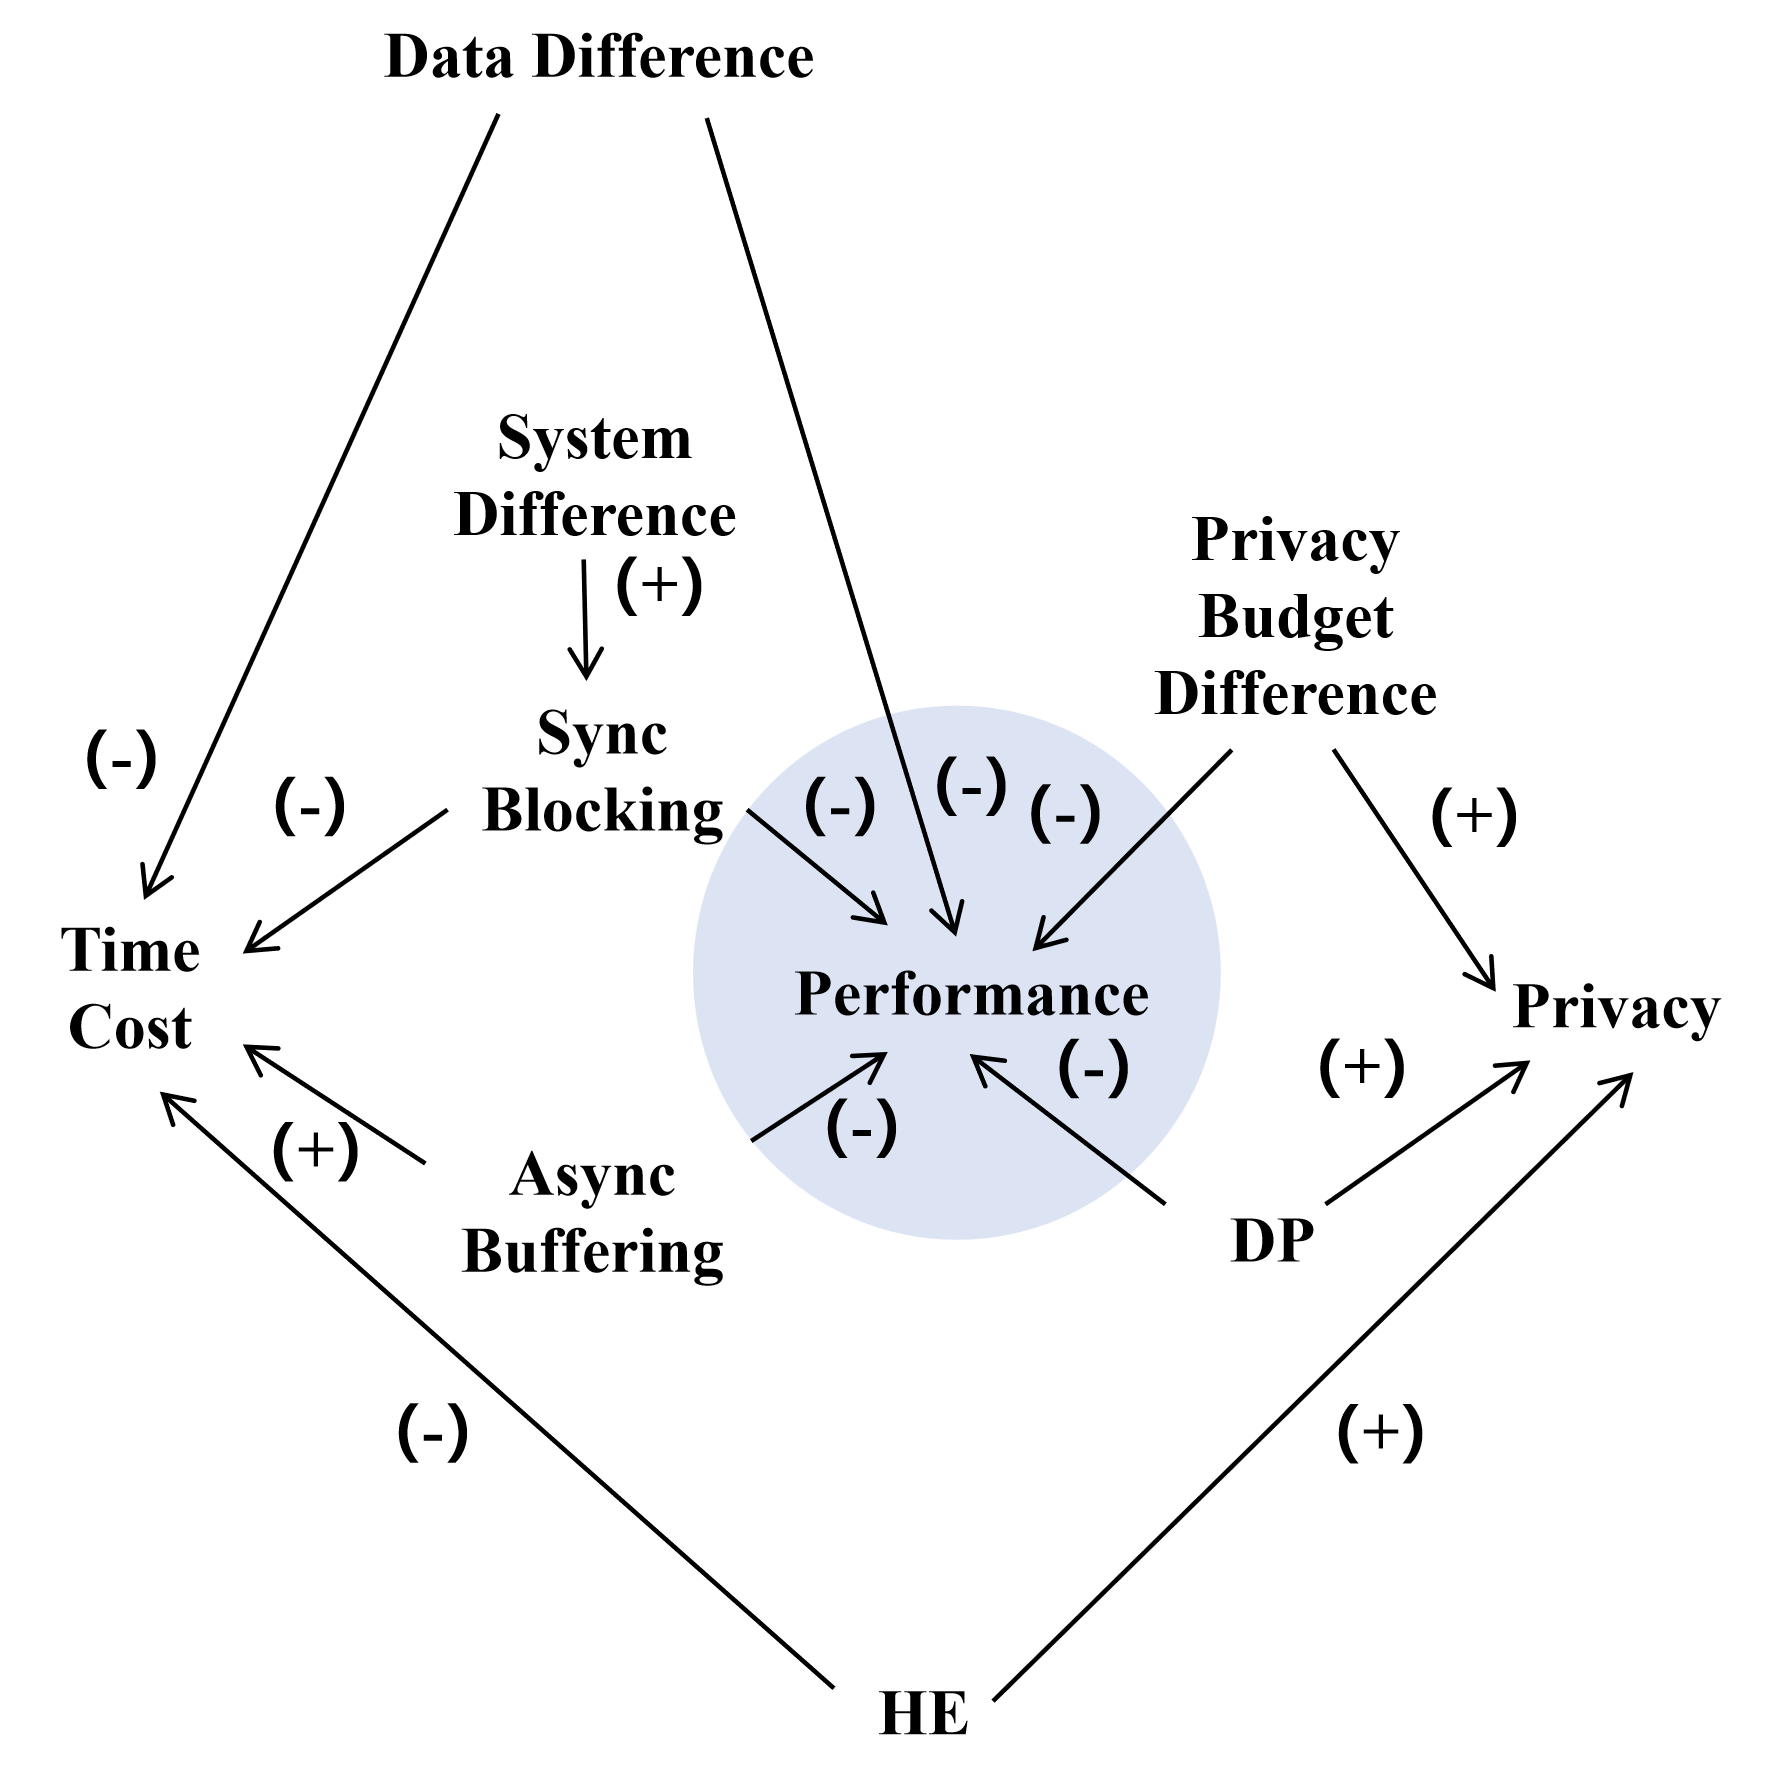
\includegraphics[width=0.78\columnwidth]{balance.png}
\caption{Coupled tradeoff among privacy protection, training utility, and efficiency.}
\label{fig:balance}
\end{figure}

This paper studies round-wise reconfiguration of cloud-edge-end federated
learning under heterogeneous resources and evolving privacy state. At each
selection round, the system evaluates feasible collaboration and protection
profiles under the current conditions rather than enforcing one collaboration
workflow for all clients. The main contributions are summarized as follows.
\begin{itemize}
    \item We formulate cloud-edge-end collaboration as a seven-mode execution space that includes edge-only, direct-cloud, and edge-to-cloud training and aggregation paths. The selected mode determines the actual communication and aggregation topology of the client in that round.
    \item We model privacy from the resulting exposure. Mode-specific transmissions determine the protection requirements; cloud-facing update releases use distinct DP and HE roles, and dynamic DP uses a state-dependent, lifetime-aware minimum feasible noise calibration rather than discrete multiplicative noise tiers.
    \item We jointly model system latency and estimated convergence-error cost for a global collaboration profile. Candidate-specific DP distortion enters the error-cost estimate, while resource and privacy requirements define hard feasibility conditions.
    \item We solve the resulting two-objective reconfiguration problem with a bounded non-dominated Pareto archive and an ideal-point Tchebycheff criterion normalized over the current archive. The experimental design separately evaluates fixed and dynamic collaboration and privacy policies.
\end{itemize}

\section{Related Work}
\label{sec:related_work}
\subsection{HFL Under Heterogeneous Environments}
HFL introduces edge servers between end devices and the cloud to reduce direct cloud communication pressure through edge pre aggregation~\cite{hfl}.
Resource aware FL studies reduce stragglers and communication overhead by adjusting client selection, local update frequency, pruning, and model compression under limited computation, energy, and bandwidth resources~\cite{phfl,xu2022adaptive,wang2019adaptivefl,dinh2021wirelessfl}.
Personalized HFL further mitigates performance degradation under non-IID data through edge side personalized models, similarity aggregation, and model decoupling~\cite{Personalizedhfl,JSJX202502007}.
These methods show that HFL can improve training from resource scheduling, communication control, and data heterogeneity adaptation.
However, when end device resources differ across computation, memory, and communication capabilities, using the same training flow for all clients can still cause straggler blocking in conventional synchronous aggregation and prevent weak devices from participating effectively.
This paper jointly considers end device computation constraints, memory constraints, communication overhead, and model split positions during collaboration reconfiguration.
Dynamic selection itself may also introduce reconfiguration overhead. Recent multi job FL studies explicitly model switching cost in client selection and reduce it through block wise selection, where the selected client subset is kept unchanged across multiple rounds~\cite{CHEN2026112204,10757319}. This observation motivates the use of a strategy update period in our framework. Collaborative modes are re evaluated only at update points, which limits unnecessary mode reconfiguration while preserving adaptability to resource and link changes.

\subsection{Cloud-Edge-End Collaborative Federated Learning}
HFL is a representative form of cloud-edge-end collaborative FL, in which end devices, edge nodes, and the cloud jointly execute computation, aggregation, and communication tasks.
As model size and system heterogeneity increase, fixed full end device training followed by edge aggregation becomes less suitable for resource limited IoT devices.
FedAgg~\cite{BSBODP} uses bridge samples and online distillation to enable models of different scales at the end, edge, and cloud layers to collaborate.
SFETEC~\cite{SFETEC} introduces split federated learning into Thing Edge Cloud environments and partitions model computation across layers to reduce end device computation load.
Cloud-edge-end task offloading studies also combine FL, privacy protection, and task efficiency~\cite{dong2026privacyoffloading}.
These studies show the value of collaboration among the three layers, but they usually assume a fixed collaboration structure.
In contrast, this paper studies how each device should select a collaborative mode under given resource and privacy conditions.
The need to balance reconfiguration gain and reconfiguration cost is also consistent with edge computing task migration studies. In mobile edge computing, migration can reduce service delay when users move away from the original edge server, but it also consumes backhaul transmission and reconfiguration resources~\cite{ZHANG2019111}. Load aware task migration further models migration cost as a combination of communication, queuing, and computation costs, and notes that migration cost can be related to physical distance between edge nodes~\cite{ZHU2024303}. These studies suggest that dynamic cloud-edge-end collaboration should account for both the benefit of changing execution paths and the overhead caused by such changes.

\subsection{Privacy Preserving HFL}
Model parameters, gradients, and intermediate representations in federated training may leak information about private data.
Differential privacy (DP), homomorphic encryption (HE), and secure aggregation are therefore widely used in FL.
For HFL, group local DP provides personalized privacy through sampling, randomized response, and shuffling~\cite{GLDP}.
Adaptive DP FL improves convergence and model utility through dynamic privacy budget allocation, adaptive clipping, and client selection~\cite{xu2025adpfl}.
Other privacy preserving HFL studies combine client level DP, secure aggregation, and CKKS style HE for data space scenarios~\cite{PPHFL}. Related fog FL studies combine hierarchical aggregation, personalization, and DP for IoT intrusion detection~\cite{islam2025pphffl}.
These studies mainly focus on the security guarantee, budget allocation, and accuracy degradation of a particular privacy mechanism.
The joint modeling of privacy induced communication cost, computation latency,
estimated convergence error cost, and cloud-edge-end collaboration reconfiguration remains
insufficiently studied.

\begin{table*}[t]
\centering
\caption{Representative Capability Comparison}
\label{tab:capability_comparison}
\small
\setlength{\tabcolsep}{4pt}
\begin{tabularx}{\textwidth}{@{}lXXXXX@{}}
\hline
\textbf{Method category} & \textbf{Execution placement} & \textbf{Aggregation topology} & \textbf{Transmitted objects} & \textbf{Privacy mechanisms} & \textbf{Joint reconfiguration} \\
\hline
Conventional HFL~\cite{hfl} & Fixed & Fixed hierarchy & Model update & Not a decision & No \\
Resource aware FL~\cite{wang2019adaptivefl,dinh2021wirelessfl} & Fixed & Fixed & Model update & Not a decision & No \\
Split cloud-edge-end FL~\cite{SFETEC} & Fixed split & Fixed & Feature, gradient, update & Not a decision & No \\
Privacy preserving HFL~\cite{GLDP,PPHFL} & Fixed & Fixed & Mechanism specific & DP or HE in a fixed workflow & No \\
Proposed framework & Adaptive & Adaptive & Feature, gradient, update & Joint DP and HE decision & Yes \\
\hline
\end{tabularx}
\end{table*}

The added capability is the joint reconfiguration of a complete federated
learning workflow. Existing categories optimize selected resources, training
steps, or privacy parameters within a prescribed collaboration structure. The
proposed collaboration space instead makes complete workflows with different
execution locations, aggregation paths, transmitted objects, and privacy
mechanisms comparable under one feasible decision model.

\section{Model Construction}
\label{sec:model}
\subsection{Cloud-Edge-End Collaborative Link Modeling}
\label{sec:link_model}
We consider a three-tier federated learning system composed of end devices,
edge nodes, and one cloud node. Let \(\mathcal N\) denote the set of end devices.
At round \(t\), an admitted device \(i\) executes one collaboration mode
\(h_i^t\) from
\begin{equation}
\mathcal H=\{\mathrm{LIE},\mathrm{LIIE},\mathrm{LIC},\mathrm{LIIC},
\mathrm{LIEIIC},\mathrm{LIEIIIC},\mathrm{LIIEIIIC}\}.
\label{eq:seven_modes}
\end{equation}
All seven modes are executable candidates. A mode specifies where computation is
performed, which objects are transmitted between the end, edge, and cloud
layers, where aggregation occurs, and how the resulting model state is returned.
Thus, the mode determines the physical information flow before a privacy
mechanism is assigned.

Given global model \(M^t\), a split mode may induce model blocks executed at the
end, edge, and cloud, denoted by \(M_L^{h_i}\), \(M_E^{h_i}\), and
\(M_C^{h_i}\), respectively. A local-update mode instead completes the local
training step before transmitting an update to its aggregation layer. Raw
training samples remain on the end device in every mode.

\begin{definition}[Mode-induced transmission set]
For device \(i\), round \(t\), and mode \(h\), let
\begin{equation}
\mathcal X_i^t(h)=\{(u,v,b,n):\text{mode }h\text{ sends object }b
\text{ from }u\text{ to }v\text{ }n\text{ times}\},
\end{equation}
where \(u,v\in\{L,E,C\}\) and
\(b\in\{\mathrm{emb},\mathrm{logits},\mathrm{grad},\mathrm{emb\_grad},\mathrm{upd}\}\).
The set records the communication/exposure topology used by the cost and
protection models. Model-return transmissions are included in the physical flow
but do not by themselves create a DP release.
\end{definition}

The seven modes have the following physical meanings. LIE performs split
training between the end and edge and terminates its aggregation path at the
edge. LIIE trains locally and submits an update to the edge. LIC performs split
training directly between the end and cloud. LIIC trains locally and submits an
update directly to the cloud. LIEIIC performs end-edge split training and then
submits the edge-side update to the cloud. LIEIIIC repeats the end-edge split
stage before the edge update is submitted to the cloud, while LIIEIIIC repeats
the local-update/edge stage before the edge update is submitted to the cloud.
In the current implementation, the two repeated-stage modes use
\(E_B=3\) edge-stage loops.

\begin{table*}[t]
\centering
\caption{Cloud-Edge-End Collaboration Modes}
\label{tab:collaboration_modes}
\small
\setlength{\tabcolsep}{4pt}
\begin{tabular}{llll}
\hline
\textbf{Mode} & \textbf{Primary training path} & \textbf{Aggregation path} & \textbf{Cloud-facing update exposure} \\
\hline
LIE & End--Edge split & Edge & No \\
LIIE & Local training & Edge & No \\
LIC & End--Cloud split & Cloud & No model-update upload \\
LIIC & Local training & Cloud & \(L\!\rightarrow\!C:\mathrm{upd}\) \\
LIEIIC & End--Edge split & Edge then Cloud & \(E\!\rightarrow\!C:\mathrm{upd}\) \\
LIEIIIC & Repeated End--Edge split & Edge then Cloud & \(E\!\rightarrow\!C:\mathrm{upd}\) \\
LIIEIIIC & Repeated local/Edge stage & Edge then Cloud & \(E\!\rightarrow\!C:\mathrm{upd}\) \\
\hline
\end{tabular}
\end{table*}

For compatibility with the link-level latency model, define the transmission
indicator
\begin{equation}
\mathbf I_b^h(u,v)=
\begin{cases}
1,&\text{if }\mathcal X_i^t(h)\text{ contains a transmission of }b\text{ from }u\text{ to }v,\\
0,&\text{otherwise}.
\end{cases}
\end{equation}
The indicator states only whether the physical transmission exists; it does not
assign one fixed privacy mechanism to the mode.

After \(\mathcal X_i^t(h)\) is known, the privacy requirement determines the
protection map \(\pi_i^t\). In the formal paper profile, lifetime DP accounting is
update-level: cloud-facing update links that require formal protection are
\(L\!\rightarrow\!C:\mathrm{upd}\) and \(E\!\rightarrow\!C:\mathrm{upd}\).
These protected update exposures require DP calibration and encrypted
aggregation, whereas feature/gradient transmissions are not counted as formal
lifetime DP events in the current implementation. DP and HE therefore have
distinct roles: DP controls privacy loss of the calibrated update release, while
HE protects update confidentiality during the required encrypted aggregation.
The detailed calibration and accounting rules are introduced in the privacy
subsection.

The link graphs in \figref{fig:eecblockflow} illustrate the seven physical mode
templates. Unlike a common release overlay, these paths are executed according
to the selected mode itself; an edge-only mode remains edge-only, while a
cloud-reaching mode follows its corresponding direct or edge-to-cloud path.
\begin{figure*}[t]
\centering
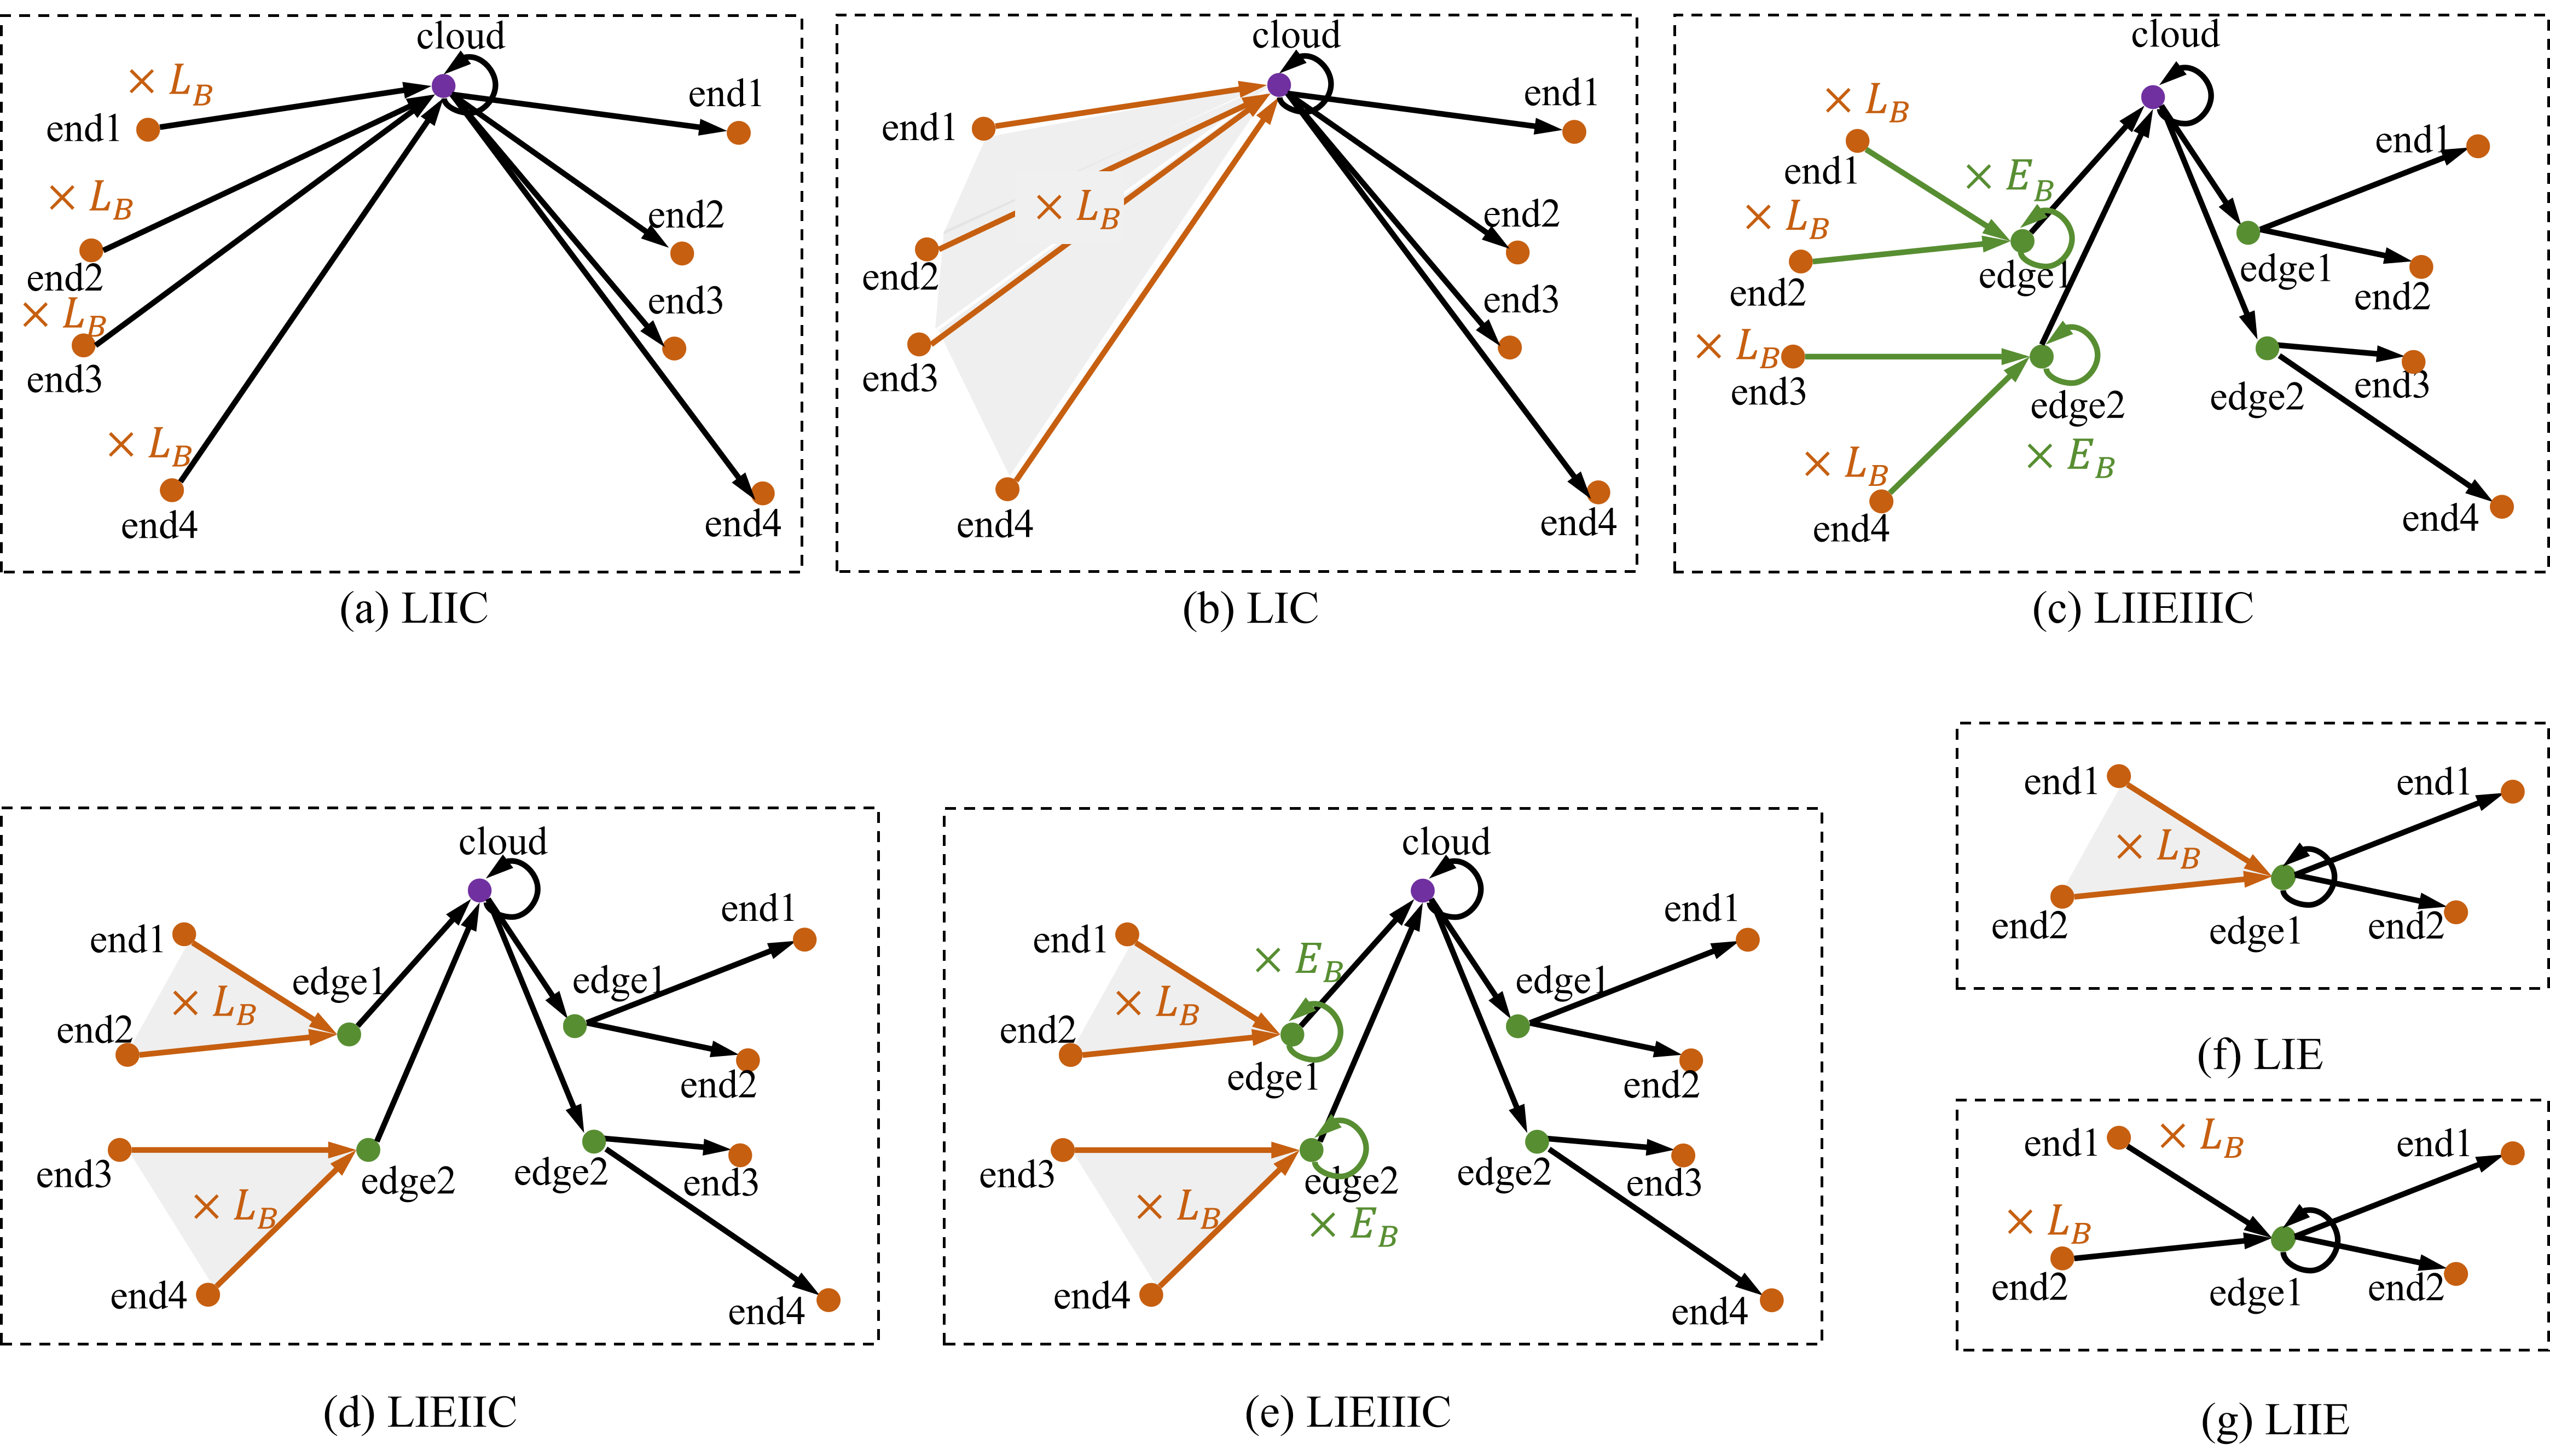
\includegraphics[width=\textwidth]{eecblockflow.png}
\caption{Cloud-edge-end collaborative link graphs of the seven collaborative modes.}
\label{fig:eecblockflow}
\end{figure*}

\subsection{Joint Cost and Utility Modeling}
\label{sec:cost_utility_model}
After the link topology is determined, a mode determines the transmissions that are physically exposed in the current round. The protection map is then generated from those exposures and the client privacy requirement. Thus, mode generation precedes mechanism assignment, while the resulting mode--protection candidate is evaluated jointly.
The selected mode must satisfy the computation and memory limits of the end device, and every protected exposure must satisfy its mechanism and lifetime privacy constraints. The joint candidate profile then determines the system-level latency and estimated convergence-error cost.
The modeling below is organized in five parts: end-side resource feasibility, path-level latency, buffered aggregation cost, exposure-specific privacy feasibility, and convergence-error cost estimation.

\subsubsection{End Side Resource Feasibility}
Let \(n_i\) be the number of local samples processed by device \(i\) in one round, and let \(L_B\) be the number of local link block iterations.
Under mode \(h_i\), \(\chi(h_i)\) denotes the profiled computation workload required by the end layer to process one sample.
The subscript \(L\) denotes the local end device layer.
The single round local computation workload is
\(W_{i,L}^{\mathrm{comp}}(h_i)=L_Bn_i\chi(h_i)\).

The value of \(\chi(h_i)\) depends on the model blocks assigned to the end device and is obtained through offline profiling.
When detailed operator level profiling is unavailable, it is approximated as
\(\chi(h_i)\approx\kappa_cm_i(h_i)\), where \(m_i(h_i)\) is the parameter
scale assigned to device \(i\), and \(\kappa_c\) is a calibrated conversion
coefficient.
This provides a lightweight complexity estimate for candidate mode screening and is in line with resource aware FL latency models~\cite{zhou2023joint}.

Let \(F_i\) denote the effective computing rate of device \(i\). The end side
computation latency is
\(T_{i,L}^{\mathrm{comp}}(h_i)=W_{i,L}^{\mathrm{comp}}(h_i)/F_i\).
This follows the common wireless FL latency model, where local computation time depends on local iterations, local data size, per sample computation workload, and device computing rate.
Given the maximum allowable computation time \(\tau_i^{\max}\), the
computation budget is \(Q_{\mathrm{comp},i}=F_i\tau_i^{\max}\).

The memory requirement under mode \(h_i\) is
\(M_i^{\mathrm{mem}}(h_i)=s_{\mathrm{state}}m_i(h_i)+a_i(h_i)\).
This model follows the common separation between parameter related model states and residual training memory~\cite{3433701.3433727}.
Here, \(s_{\mathrm{state}}\) is the profiled per parameter model state memory coefficient, covering parameters, gradients, optimizer states such as Adam momentum and variance, and other persistent training states such as mixed precision parameter copies.
The term \(a_i(h_i)\) denotes residual memory that is not captured by the parameter scale, including activations and temporary training buffers.

Let \(Q_{\mathrm{mem},i}\) denote the available memory of device \(i\).
The resource feasible mode set is
\begin{equation}
    \mathcal{H}_i^{\mathrm{res}}=
    \{h_i\in\mathcal{H}\mid
    W_{i,L}^{\mathrm{comp}}(h_i)\le Q_{\mathrm{comp},i},
    M_i^{\mathrm{mem}}(h_i)\le Q_{\mathrm{mem},i}\}.
\label{eq:resource_feasible}
\end{equation}

\subsubsection{Path Level Latency}
We first define the general link and path latency terms. A representative complete path is then illustrated in \figref{fig:time}.
Let \(R^t=(R_{u,v}^t)_{u,v\in\mathcal{V}}\) be the cloud-edge-end link rate matrix in round \(t\).
The communication model is link specific. For an end edge pair \((i,j)\), the rate \(R_{i,j}^{t}\) and the base latency \(T_{i,j}^{0}\) may differ from those of other device edge pairs. These parameters capture heterogeneous physical distance, wireless channel quality, interference, and congestion. Therefore, two end devices connected to the same edge server can have different communication latencies, and the same device connected to different edge servers can also experience different communication latencies~\cite{ZHANG2019111,ZHU2024303}.
For an interaction link \(\lambda=(u,v,b)\), its raw transmission size is \(S_{\lambda}^t(h_i)\).
Let \(\psi_{\lambda}(h_i,\pi_i)\) denote the actual protection/transport mechanism on link \(\lambda\) under mode \(h_i\). The map \(\pi_i\) is generated only after the mode-specific transmissions and their protection requirements are known. It uses \(\mathrm{none}\) for links that do not require protection, including model-return links in the current paper profile.
\begin{equation}
\psi_{\lambda}(h_i,\pi_i)=
\begin{cases}
\pi_i(\lambda), & \lambda\in\mathcal{E}_{\mathrm{priv}}^{h_i},\\
\mathrm{none}, & \lambda\notin\mathcal{E}_{\mathrm{priv}}^{h_i}.
\end{cases}
\end{equation}
Thus, a model return link uses \(\mathrm{none}\) even when its object type is
\(\mathrm{upd}\). The effective transmission size is
\(\widetilde{S}_{\lambda}^t(h_i,\pi_i)=
\alpha(\psi_{\lambda}(h_i,\pi_i))S_{\lambda}^t(h_i)\), where
\(\alpha(\cdot)\) is the communication inflation factor induced by the
fixed induced protection mechanism.
For \(\mathrm{none}\), \(\alpha(\mathrm{none})=1\).
For DP, \(\alpha(\mathrm{DP})\approx 1\). For HE, ciphertext encoding and packing increase the transmitted payload, so \(\alpha(\mathrm{HE})>1\)~\cite{PPHFL}.
In practice, \(\alpha(\mathrm{HE})\) can be obtained by offline profiling as the ratio between the serialized ciphertext payload size and the original plaintext tensor size.
The communication latency is
\begin{equation}
T_{\lambda}^{\mathrm{link},t}(h_i,\pi_i)
=
\frac{\widetilde{S}_{\lambda}^t(h_i,\pi_i)}
{R_{\lambda}^{t}}
+D_{\lambda}^{0}+T_{\lambda}^{\mathrm{priv},t}(\psi_{\lambda}(h_i,\pi_i)),
\label{eq:comm_latency}
\end{equation}
where \(R_{\lambda}^{t}=R_{u,v}^{t}\) for \(\lambda=(u,v,b)\), \(D_{\lambda}^{0}\) is the fixed base delay, and \(T_{\lambda}^{\mathrm{priv},t}\) is the link endpoint privacy processing latency. For \(\mathrm{none}\), \(T_{\lambda}^{\mathrm{priv},t}(\mathrm{none})=0\). Round level network fluctuation is represented by the time varying link rate \(R_{u,v}^{t}\).

Using this link level term, the path level link flow latency of end device \(i\), denoted by \(T_i^t(h_i,\pi_i)\), is decomposed into execution, communication, waiting, aggregation, and switching components.

The transmission indicator matrices build the communication part of the link
flow as \(\mathcal{E}_{\mathrm{flow}}^{h_i}=
\{\lambda=(u,v,b)\mid b\in\mathcal{B},\
\mathbf{I}_{b}^{h_i}(u,v)=1\}\).
Thus, nonzero entries in \(\mathbf{I}_{b}^{h_i}\) identify the communication links induced by mode \(h_i\).
The subset \(\mathcal{E}_{\mathrm{priv}}^{h_i}\) contains the links in \(\mathcal{E}_{\mathrm{flow}}^{h_i}\) that require privacy protection.
Let \(N_{\lambda}(h_i)\) be the number of times link \(\lambda\) is executed in one complete link flow.
For a link executed inside a local link block, \(N_{\lambda}(h_i)=L_B\).
If the local link block is nested inside an edge aggregation loop, the count becomes \(N_{\lambda}(h_i)=L_BE_B\).
For links executed once per edge aggregation loop, \(N_{\lambda}(h_i)=E_B\).
For final aggregation upload and model return links outside repeated loops, \(N_{\lambda}(h_i)=1\).
The path level latency is decomposed as
\begin{equation}
\begin{aligned}
T_i^t(h_i,\pi_i)
&=T_i^{\mathrm{exec},t}(h_i)
+\sum_{\lambda\in\mathcal{E}_{\mathrm{flow}}^{h_i}}
N_{\lambda}(h_i)T_{\lambda}^{\mathrm{link},t}(h_i,\pi_i)\\
&\quad +T_i^{\mathrm{wait},t}(h_i)
+T_i^{\mathrm{agg},t}(h_i,\pi_i)
+T_i^{\mathrm{sw},t}.
\end{aligned}
\label{eq:latency_model}
\end{equation}
Here, \(T_i^{\mathrm{exec},t}\) denotes only the computation latency of the submodels executed at the end, edge, and cloud layers.
It is coupled with the selected link flow through \(h_i\), but it does not include cross layer transmission delay. That delay is accounted for separately by the summation of \(T_{\lambda}^{\mathrm{link},t}\) over \(\mathcal{E}_{\mathrm{flow}}^{h_i}\).
\(T_i^{\mathrm{wait},t}\) denotes the waiting latency before upper layer aggregation is triggered, and \(T_i^{\mathrm{agg},t}\) denotes the aggregation latency assigned to the link flow.
Changing the collaborative mode may require execution path rescheduling and model state movement, similar to task migration and switching cost modeling in edge computing and wireless FL~\cite{ZHANG2019111,ZHU2024303,CHEN2026112204,10757319,li2026latency}.
The term \(T_i^{\mathrm{sw},t}\) denotes this mode reconfiguration latency in round \(t\), and we model it as
\begin{equation}
T_i^{\mathrm{sw},t}
=\eta_h \mathbb{I}(h_i^t\neq h_i^{t-1})
+\eta_p
\frac{\|\mathbf{p}(h_i^t)-\mathbf{p}(h_i^{t-1})\|_1}{2},
\label{eq:switching_cost}
\end{equation}
where \(\eta_h\ge 0\) is the fixed time cost incurred when the selected collaborative mode changes, similar to the unit switching cost used in dynamic FL client selection~\cite{CHEN2026112204}.
\(\eta_p\ge 0\) is the maximum variable time cost associated with model state placement change, motivated by edge service migration models where migration cost is proportional to the migrated service state size~\cite{li2026latency}.
Both coefficients are configurable or profile based system parameters.
To quantify the placement-change term in \(T_i^{\mathrm{sw},t}\), we define the normalized model state placement vector of mode \(h\) as
\begin{equation}
\mathbf{p}(h)=
\frac{1}{Z_h}
\left[
\lvert M_L^h\rvert,
\lvert M_E^h\rvert,
\lvert M_C^h\rvert
\right],
\label{eq:model_placement_vector}
\end{equation}
where \(Z_h=\lvert M_L^h\rvert+\lvert M_E^h\rvert+\lvert M_C^h\rvert\). \(M_L^h\), \(M_E^h\), and \(M_C^h\) are the model state portions placed at the end, edge, and cloud layers under mode \(h\), respectively, and \(\lvert\cdot\rvert\) denotes profiled model state size. This normalization gives \(\mathbf{1}^{\top}\mathbf{p}(h)=1\), so \(\|\mathbf{p}(h_i^t)-\mathbf{p}(h_i^{t-1})\|_1/2\in[0,1]\). The normalized distance estimates the fraction of model state whose placement changes between two consecutive selected modes.

\subsubsection{Buffered Aggregation Cost}
This subsection specifies the waiting and aggregation terms used in the path latency model under buffered aggregation.
To mitigate synchronization blocking caused by slow devices, aggregation is
triggered after the required number of updates has arrived.
For edge aggregator \(j\), let \(N_j\) be the number of associated end devices and \(\rho_{\mathrm{buf}}\in(0,1]\) be the buffered aggregation participation threshold.
The number of clients needed to trigger aggregation is \(K_j=\lceil\rho_{\mathrm{buf}} N_j\rceil\).
Let \(T_i^{\mathrm{lupd}}\) be the time needed for device \(i\) to complete the collaborative update process before upload.
Let \(T_{i,j}^{\mathrm{comm},t}(h_i,\pi_i)\) denote the communication latency of the update upload from device \(i\) to edge aggregator \(j\), obtained from \(T_{\lambda}^{\mathrm{link},t}\) for the corresponding link \(\lambda=(i,j,\mathrm{upd})\).
The arrival time at edge \(j\) is
\(x_{i,j}^t=T_i^{\mathrm{lupd}}(h_i,\pi_i)+
T_{i,j}^{\mathrm{comm},t}(h_i,\pi_i)\).
Sorting arrival times as \(x_{(1),j}^t\le\cdots\le x_{(N_j),j}^t\), let
\(S_j^t(\mathbf x)=\{i_{(1)},\ldots,i_{(K_j)}\}\) be the first \(K_j\) arrived clients
selected into the buffered aggregation. The edge aggregation starts at
\(X_j^t(\mathbf x)=x_{(K_j),j}^t=\max_{i\in S_j^t(\mathbf x)}x_{i,j}^t\), and client \(i\) waits
\(W_{i,j}^{\mathrm{agg},t}=\max(0,X_j^t(\mathbf x)-x_{i,j}^t)\).
If multiple updates arrive exactly at the trigger time \(X_j^t(\mathbf x)=x_{(K_j),j}^t\), all tied updates are admitted, so \(\lvert S_j^t(\mathbf x)\rvert\) may exceed \(K_j\).
The edge aggregation time is
\(T_j^{\mathrm{agg},t}=\beta_j\sum_{i\in S_j^t(\mathbf x)}
\widetilde{S}_{i,j}^{\mathrm{upd},t}+T_j^{\mathrm{fix}}\), where \(\beta_j\)
is the aggregation processing coefficient of edge aggregator \(j\). For the
update upload link \(\lambda=(i,j,\mathrm{upd})\),
\(\widetilde{S}_{i,j}^{\mathrm{upd},t}=\widetilde{S}_{\lambda}^t(h_i,\pi_i)\),
i.e., the effective payload size of client \(i\)'s update received by edge
aggregator \(j\) after the selected protection mechanism is applied. The
coefficient \(\beta_j\) can be obtained by offline profiling with varying
update counts and payload sizes, and \(T_j^{\mathrm{fix}}\) denotes the fixed
aggregation overhead. Protection processing, including HE encryption/decryption overhead on protected update paths, is accounted for in the
link endpoint term \(T_{\lambda}^{\mathrm{priv},t}\).

The same construction is applied to every aggregation group induced by a
complete candidate profile
\(\mathbf x=\mathbf h_{\mathcal N}\). The protection map is generated from each selected mode and its exposure requirements. Clients are grouped by their
selected aggregation endpoint and compatible link flow. Each edge buffer
admits its earliest required arrivals. An admitted edge aggregate that reaches
the cloud then becomes a cloud arrival, and the cloud buffer applies the same
rule to its incoming client or edge objects. Let \(A_i^t(\mathbf x)\) denote
the source clients admitted to the buffer associated with client \(i\)'s
selected path under profile \(\mathbf x\), and let
\(A^t(\mathbf x)=\bigcup_i A_i^t(\mathbf x)\) be the complete admitted client
set. The system latency \(T_{\mathrm{sys}}^t(\mathbf x)\) is the latest
completion time of the triggered terminal aggregation and model return events.
The link rates, resource state, topology, and previous profile are fixed during
one evaluation, while \(\mathbf x\) determines the path choices and arrival
times. Therefore, every candidate profile produces its own
\(A_i^t(\mathbf x)\) and \(T_{\mathrm{sys}}^t(\mathbf x)\). When
\(\rho_{\mathrm{buf}}=1\), every active buffer waits for all its members and
the same procedure reduces to full admission.
\begin{figure}[t]
\centering
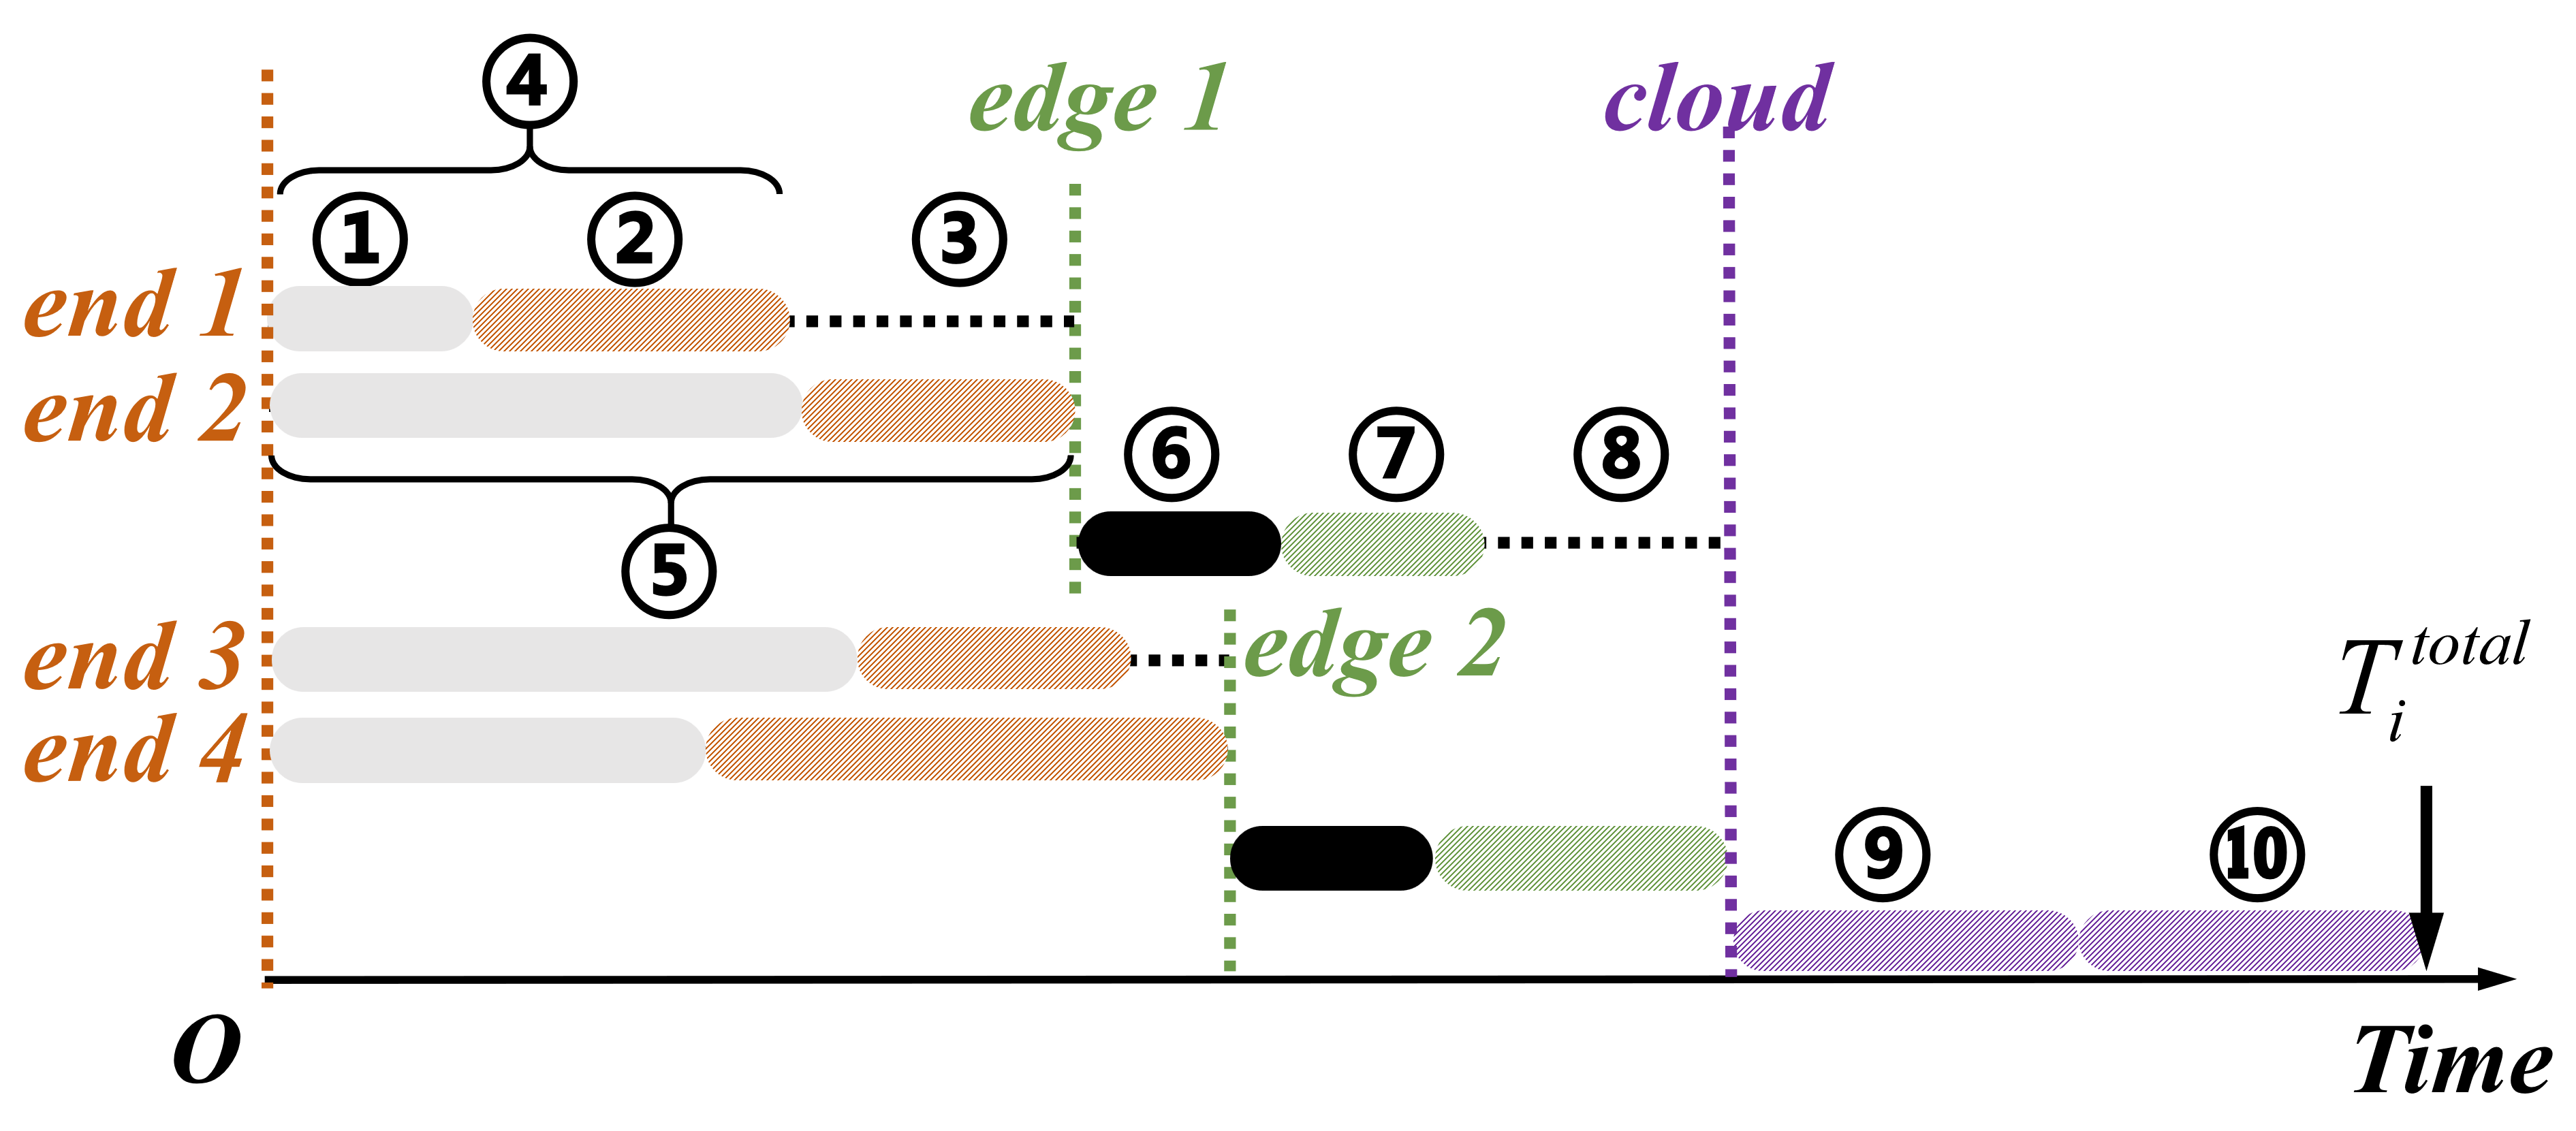
\includegraphics[width=\columnwidth]{time.png}
\caption{Path level link flow latency decomposition for an end device in cloud-edge-end collaborative FL.}
\label{fig:time}
\end{figure}

Fig.~\ref{fig:time} illustrates how the general latency decomposition in \equref{eq:latency_model} is instantiated in a representative complete end-edge-cloud link flow.
The directional communication terms in the figure, such as \(T_{i,j}^{\mathrm{comm},t}\), \(T_{j\rightarrow c}^{\mathrm{comm},t}\), \(T_{c\rightarrow j}^{\mathrm{comm},t}\), and \(T_{j\rightarrow i}^{\mathrm{comm},t}\), are shorthand instances of \(T_{\lambda}^{\mathrm{link},t}\) for the corresponding directed links and transmitted objects.
Marker \textcircled{1} denotes the local model training time of the end device, corresponding to \(T_i^{\mathrm{lupd}}(h_i,\pi_i)\).
Marker \textcircled{2} denotes the communication time for uploading the transmission object of the selected link flow to the associated edge server, corresponding to \(T_{i,j}^{\mathrm{comm},t}(h_i,\pi_i)\). The transmission object is determined by \(b\in\mathcal{B}\).
Marker \textcircled{3} denotes the waiting time after the upload is completed and before the edge server starts aggregation, corresponding to \(W_{i,j}^{\mathrm{agg},t}\).
Marker \textcircled{4} denotes the arrival time \(x_{i,j}^{t}\) at the edge server.
Marker \textcircled{5} denotes the start time \(X_j^{t}(\mathbf x)\) of local edge aggregation, which is determined by the latest arrival among the selected buffered aggregation set \(S_j^t(\mathbf x)\).
Marker \textcircled{6} denotes the edge aggregation time, corresponding to \(T_j^{\mathrm{agg},t}\).
Marker \textcircled{7} denotes the communication time for uploading the edge aggregated model to the cloud server, corresponding to \(T_{j\rightarrow c}^{\mathrm{comm},t}\).
Marker \textcircled{8} denotes the waiting time after the edge server completes uploading and before the cloud server starts global aggregation, corresponding to \(W_{j,c}^{\mathrm{agg},t}\).
Marker \textcircled{9} denotes the cloud global aggregation and model return stage, including the cloud aggregation time \(T_c^{\mathrm{agg},t}\) and the cloud to edge download time \(T_{c\rightarrow j}^{\mathrm{comm},t}\).
Marker \textcircled{10} denotes the communication time for returning the updated global model from the edge server to the end device, corresponding to \(T_{j\rightarrow i}^{\mathrm{comm},t}\).

For this representative path, \(T_i^t(h_i,\pi_i)\) can be expanded as
\begin{equation}
\begin{aligned}
T_i^t(h_i,\pi_i)
=&\;
T_i^{\mathrm{lupd}}(h_i,\pi_i)
+T_{i,j}^{\mathrm{comm},t}(h_i,\pi_i)
+W_{i,j}^{\mathrm{agg},t}
+T_j^{\mathrm{agg},t}\\
&+T_{j\rightarrow c}^{\mathrm{comm},t}
+W_{j,c}^{\mathrm{agg},t}
+T_c^{\mathrm{agg},t}
+T_{c\rightarrow j}^{\mathrm{comm},t}
+T_{j\rightarrow i}^{\mathrm{comm},t}.
\end{aligned}
\label{eq:path_total_latency}
\end{equation}
The expanded form is shown only for the representative path in \figref{fig:time}. For any selected mode \(h_i\), \(T_i^t(h_i,\pi_i)\) accumulates the terms on the complete link flow induced by that mode, including the model return required to prepare the device for the next round.

\subsubsection{Exposure-Specific Privacy Protection and Lifetime Accounting}
\label{sec:privacy_model}
The privacy mechanism is assigned to the transmissions created by a candidate mode rather than to a mode label itself. For client $i$ in round $t$, let
\begin{equation}
\mathcal X_i^t(h)=\{(\lambda,b,N_\lambda(h))\}
\label{eq:mode_exposure_set}
\end{equation}
denote the mode-specific transmission set, where $\lambda$ is a directed link, $b\in\mathcal B$ is the transmitted object, and $N_\lambda(h)$ is its execution count. A client requirement specifies which members of $\mathcal X_i^t(h)$ forbid plaintext transmission and which require DP. The protection map $\pi_i^t$ is legal only when every exposed link satisfies these requirements.

The current paper profile protects model updates exposed to the Cloud. In particular, the update links $L\!\rightarrow\!C$ and $E\!\rightarrow\!C$ require both confidentiality and DP. Therefore, their legal protection uses HE for encrypted aggregation and DP for calibrated randomization. Feature and gradient transmissions are allowed in plaintext in the current profile and do not enter the formal lifetime DP accountant. Returned models are also not treated as new DP events. This separation is important: HE protects the confidentiality of protected update contributions during aggregation, whereas DP controls the privacy loss of a calibrated release. One mechanism does not substitute for the other.

Let $\mathcal D_i^t(h)\subseteq\mathcal X_i^t(h)$ denote the update exposures that require DP, and let
\begin{equation}
n_{i,h}^{t,\mathrm{upd}}
=\sum_{x\in\mathcal D_i^t(h)}N_x(h)
\label{eq:update_dp_event_count}
\end{equation}
be the number of protected update events generated by one execution of candidate mode $h$. For the current paper profile, modes without a Cloud-facing update have $n_{i,h}^{t,\mathrm{upd}}=0$, while a Cloud-facing update path contributes the corresponding protected event count.

We maintain a client-level RDP ledger $R_{i,\mathrm{upd}}^t(\alpha)$ for the protected update events. For a Gaussian event with noise multiplier $\sigma$, the accountant adds
\begin{equation}
\Delta R_{\mathrm{upd}}(\alpha;\sigma)=\frac{\alpha}{2\sigma^2},
\label{eq:privacy_budget}
\end{equation}
and converts the accumulated RDP state to $(\epsilon,\delta_{\mathrm{upd}})$ through
\begin{equation}
\epsilon_{i,\mathrm{upd}}^t
=\min_{\alpha>1}\left[
R_{i,\mathrm{upd}}^t(\alpha)
+\frac{\log(1/\delta_{\mathrm{upd}})}{\alpha-1}
\right].
\label{eq:rdp_to_dp}
\end{equation}
The lifetime target is $\epsilon_{i,\mathrm{upd}}^t\le\bar\epsilon_{i,\mathrm{upd}}$.

Dynamic privacy is implemented by state-dependent lifetime-aware calibration. At round $t$, define the remaining planning horizon as
\begin{equation}
H_t=\max\{1,R-t\},
\label{eq:remaining_privacy_horizon}
\end{equation}
where $R$ is the configured number of training rounds under the implementation's round indexing. A candidate with $n_{i,h}^{t,\mathrm{upd}}>0$ reserves
\begin{equation}
N_{i,h}^{t,\mathrm{plan}}
=n_{i,h}^{t,\mathrm{upd}}H_t
\label{eq:planned_update_events}
\end{equation}
protected update events. Its noise multiplier is the minimum value that keeps these planned events feasible under the current ledger,
\begin{equation}
\sigma_{i,h}^t
=\sigma_{\min}\!\left(
R_{i,\mathrm{upd}}^t,
N_{i,h}^{t,\mathrm{plan}},
\bar\epsilon_{i,\mathrm{upd}},
\delta_{\mathrm{upd}}
\right).
\label{eq:noise_calibration}
\end{equation}
Thus the current dynamic candidate contains one lifetime-aware feasible noise value rather than several multiplicative noise tiers. If no such value exists, the candidate is privacy-infeasible. The ledger is updated from the DP events that are actually executed and released, so the next round is calibrated from the resulting privacy state.

This accounting establishes exposure-specific, update-level client DP for the protected events represented by the ledger. It does not establish DP for all feature or gradient transmissions, and it does not by itself establish a uniform end-to-end DP guarantee for the final global model under arbitrary adaptive protocol behavior.

\subsubsection{Estimation of Convergence Error Cost}
The selector does not use future test loss, which is unavailable at decision time. Instead, it evaluates a convergence-error proxy whose local components include stochastic training variation, clipping distortion, and the DP distortion generated by the candidate-specific update noise multiplier.

For a candidate $x_i^t=(h_i^t,\pi_i^t)$, let $n_{i,c}^t$ and $n_{i,e}^t$ denote the protected update-DP event counts attributed to client-side and edge-side update aggregation, respectively. Let $C_u$ be the update clipping norm, $d$ the update dimension, $\eta_{\mathrm{lr}}$ the learning rate, and $L_B$ the local-cycle count. The update-noise variance term used by the selector has the form
\begin{equation}
V_{i,\mathrm{upd}}^t
=
\frac{(\sigma_{i,h_i}^t)^2(2C_u)^2d}
{\eta_{\mathrm{lr}}^2L_B^2}.
\label{eq:update_dp_noise_cost}
\end{equation}
Hence a larger candidate-specific $\sigma_{i,h_i}^t$ produces a larger current-round distortion term. With $\mathcal B_{\mathrm{clip},i}^t$ denoting the profiled squared clipping excess in the same gradient-unit scale, the implementation groups the local proxy into client and edge bias/variance components,
\begin{equation}
\begin{aligned}
B_{i,c}^t&=\frac{3}{2\mu}\,n_{i,c}^t\mathcal B_{\mathrm{clip},i}^t,
&V_{i,c}^t&=\frac{G\eta_{\mathrm{lr}}L_B}{\mu}
\left(\sigma_{\mathrm{local}}^2+n_{i,c}^tV_{i,\mathrm{upd}}^t\right),\\
B_{i,e}^t&=\frac{3}{2\mu}\,n_{i,e}^t\mathcal B_{\mathrm{clip},i}^t,
&V_{i,e}^t&=\frac{G\eta_{\mathrm{lr}}L_B}{\mu}
 n_{i,e}^tV_{i,\mathrm{upd}}^t.
\end{aligned}
\label{eq:client_error_cost}
\end{equation}
Here $G$ is the smoothness parameter and $\mu$ is the PL parameter used by the proxy. The current paper profile has no formal feature-DP events, so feature-DP distortion does not contribute to these terms.

For a complete profile $\mathbf x$, the evaluator combines client components with represented-sample weights and combines compatible edge-aggregation components at the group level. Writing $q_i^t(\mathbf x)$ for a normalized represented-sample weight and $q_g^t(\mathbf x)$ for the corresponding edge-group weight, the system proxy can be summarized as
\begin{equation}
\begin{aligned}
\widehat\Omega_{\mathrm{sys}}^t(\mathbf x)
={}&\sum_i\left[
q_i^t B_{i,c}^t+(q_i^t)^2V_{i,c}^t
\right]\\
&+\sum_{g\in\mathcal G_E^t(\mathbf x)}\left[
q_g^t B_{g,e}^t+(q_g^t)^2V_{g,e}^t
\right]
+\frac{\xi}{\rho_C^t(\mathbf x)+\varepsilon_C}.
\end{aligned}
\label{eq:global_omega}
\end{equation}
The last term penalizes insufficient Cloud-reaching represented sample mass, where $\rho_C^t(\mathbf x)$ is the Cloud fusion ratio. The exact weights and edge groups are induced by the evaluated profile and its admitted aggregation flow. Equation~\eqref{eq:global_omega} is a selection-time proxy rather than a claim that it equals the realized training loss.

Most importantly, the DP contribution in $\widehat\Omega_{\mathrm{sys}}^t$ is not a common global-release constant. It depends on the candidate through its protected update exposure count and its lifetime-aware $\sigma_{i,h_i}^t$. Privacy budget itself is not introduced as a third Pareto objective: it constrains feasibility through the ledger and affects learning cost through the calibrated DP distortion.

\subsection{Global Multi-Objective Collaborative Optimization}
\label{sec:global_optimization}
A client candidate is written as
\begin{equation}
x_i^t=(h_i^t,\pi_i^t,\sigma_{i,h_i}^t),
\label{eq:client_candidate}
\end{equation}
where the last component is present when the candidate contains a protected update-DP exposure. Candidate generation is hierarchical: the mode first determines $\mathcal X_i^t(h_i)$, the exposure requirements determine the legal protection map $\pi_i^t$, and the current privacy ledger determines the lifetime-aware noise calibration. These components are then evaluated jointly rather than selecting privacy independently after the mode decision.

Let $\mathcal F_i^t$ contain the candidates that satisfy the end-device resource constraints in \eqref{eq:resource_feasible}, the exposure-specific mechanism requirements, and the lifetime privacy constraint. A complete profile is $\mathbf x=(x_1^t,\ldots,x_N^t)$. The flow evaluator applies the shared edge/cloud aggregation and admission rules to a profile, so the system-feasible set is a subset of the Cartesian product,
\begin{equation}
\mathcal F_{\mathrm{sys}}^t\subseteq\prod_{i=1}^{N}\mathcal F_i^t.
\label{eq:global_feasible_set}
\end{equation}
An execution that is not admitted is reported as \textsc{skip}; \textsc{skip} is an execution outcome and is not an eighth collaboration mode.

For every feasible profile, the flow model produces the round duration $T_{\mathrm{sys}}^t(\mathbf x)$ rather than a simple sum of per-client latencies. The same profile produces $\widehat\Omega_{\mathrm{sys}}^t(\mathbf x)$ through \eqref{eq:global_omega}. The current selector therefore solves the two-objective problem
\begin{equation}
\underset{\mathbf{x}\in\mathcal F_{\mathrm{sys}}^t}{\operatorname{minimize}}\quad
\mathbf f^t(\mathbf{x})=
\begin{bmatrix}
T_{\mathrm{sys}}^t(\mathbf{x})\\
\widehat{\Omega}_{\mathrm{sys}}^t(\mathbf{x})
\end{bmatrix}.
\label{eq:global_multiobjective}
\end{equation}
Privacy reserve, HE cost, and communication volume are not separate Pareto objectives in the current implementation. HE and communication processing affect the path latency, while DP calibration affects feasibility and the error-cost proxy.

The non-dominated decision set is
\begin{equation}
\mathcal X_{\mathrm P}^t
=\{\mathbf{x}\in\mathcal F_{\mathrm{sys}}^t\mid
\nexists\mathbf{x}'\in\mathcal F_{\mathrm{sys}}^t,
\ \mathbf{x}'\prec\mathbf{x}\},
\label{eq:pareto_front}
\end{equation}
where $\prec$ denotes Pareto dominance with respect to the two objectives in \eqref{eq:global_multiobjective}. In the bounded solver, the maintained non-dominated archive approximates this set.

The Tchebycheff stage normalizes over the current non-dominated archive. Let $T_{\min}^t,T_{\max}^t$ and $\widehat\Omega_{\min}^t,\widehat\Omega_{\max}^t$ be the minimum and maximum objective values observed in that archive. These are normalization extrema, not physical latency or resource bounds. The normalized objectives are
\begin{equation}
\begin{aligned}
\bar T^t(\mathbf{x})&=
\frac{T_{\mathrm{sys}}^t(\mathbf{x})-T_{\min}^t}
{T_{\max}^t-T_{\min}^t+\varepsilon_n},\\
\bar\Omega^t(\mathbf{x})&=
\frac{\widehat\Omega_{\mathrm{sys}}^t(\mathbf{x})-\widehat\Omega_{\min}^t}
{\widehat\Omega_{\max}^t-\widehat\Omega_{\min}^t+\varepsilon_n}.
\end{aligned}
\label{eq:pareto_normalization}
\end{equation}
The normalized ideal point is the origin. The selected profile minimizes the largest normalized deviation,
\begin{equation}
\begin{aligned}
D_\infty^t(\mathbf{x})
&=\max\{\lvert\bar T^t(\mathbf{x})\rvert,
\lvert\bar\Omega^t(\mathbf{x})\rvert\},\\
\mathbf{x}^\star
&\in\arg\min_{\mathbf{x}\in\mathcal X_{\mathrm P}^t}
D_\infty^t(\mathbf{x}).
\end{aligned}
\label{eq:selection}
\end{equation}
The implementation resolves equal distances deterministically using system latency, then $\widehat\Omega_{\mathrm{sys}}^t$, followed by a stable profile identity. Real test accuracy is used only for experimental evaluation and is not available to the selector.

\section{Algorithm}
\label{sec:algorithm}

At each strategy update point, DynFL constructs candidates in the same order as the execution semantics. For client $i$, an executable mode $h_i$ first induces its transmission set $\mathcal X_i^t(h_i)$. The current exposure requirement then determines the legal protection map $\pi_i^t$. If the candidate contains a protected Cloud-facing update, its lifetime-aware multiplier $\sigma_{i,h_i}^t$ is obtained from \equref{eq:noise_calibration}; otherwise no update-DP event is charged for that candidate. Candidates that violate resource, protection, or lifetime privacy constraints are removed, producing $\mathcal F_i^t$. The flow evaluator subsequently determines whether a joint profile belongs to $\mathcal F_{\mathrm{sys}}^t$.

For a small instance, the exact solver evaluates all joint profiles in $\prod_i\mathcal F_i^t$ and retains the system-feasible ones. If $M=\prod_i|\mathcal F_i^t|$ profiles are enumerated and one global evaluation costs $C_{\mathrm{eval}}$, exact evaluation and Pareto filtering cost $O(MC_{\mathrm{eval}}+M\log M)$. This exponential dependence restricts exhaustive search to small-scale validation.

For full-scale selection, the bounded search initializes a profile archive and expands each retained profile by replacing one client candidate at a time. A deterministic exploration queue containing at most $K_{\mathrm B}$ evaluated intermediate profiles allows the search to pass through a temporarily dominated profile. The method maintains at most $K_{\mathrm P}$ non-dominated evaluated profiles. Because only a subset of $\mathcal F_{\mathrm{sys}}^t$ is explored, the resulting archive $\widehat{\mathcal X}_{\mathrm P}^t$ approximates the exact Pareto set $\mathcal X_{\mathrm P}^t$. The exact and approximate solvers use the same system objectives, archive normalization, and ideal-point Tchebycheff rule.

Let $K_{\mathrm{cand}}=\max_i|\mathcal F_i^t|$. Replacing one client candidate in one retained profile generates at most $N(K_{\mathrm{cand}}-1)$ neighbors. With at most $K_{\mathrm P}+K_{\mathrm B}$ retained archive/queue profiles, one expansion considers at most $L\le (K_{\mathrm P}+K_{\mathrm B})N(K_{\mathrm{cand}}-1)$ neighbors. At most $I_{\max}$ expansions therefore cost $O(I_{\max}L(C_{\mathrm{eval}}+\log L))$. The implementation caches candidate flow information and incrementally updates affected aggregation groups when evaluating one-client replacements.

The search is performed only at strategy update points determined by $S_P$. At other rounds, a previously selected profile may be reused only when it remains executable under the current state. Switching overhead is included in the evaluated flow latency. A non-admitted execution is reported as \textsc{skip}; it is not inserted into $\mathcal H$ as an additional collaboration mode.

DP and HE are enforced from the exposure requirement rather than from a common post-selection release overlay. Under the current paper profile, a Cloud-facing update requires both DP and HE: the DP multiplier is calibrated from the client's current ledger and remaining horizon, while HE protects the corresponding contribution during encrypted aggregation. Edge-only modes do not acquire an artificial Cloud release. After selection, only DP events that are actually executed and released are charged to the client ledger. Consequently, the next strategy update observes the privacy state produced by prior execution rather than a fixed global-release accountant.

\begin{breakablealgorithm}
\caption{Bounded Pareto Solver with Exposure-Specific Protection}
\label{alg:selection}
\small
\begin{algorithmic}[1]
\REQUIRE Device set $\mathcal N$, seven-mode set $\mathcal H$, per-client resource-feasible subsets $\mathcal H_i^{\mathrm{res}}$, current privacy ledgers $R_{i,\mathrm{upd}}^t(\alpha)$ and targets $(\bar\epsilon_{i,\mathrm{upd}},\delta_{\mathrm{upd}})$, round system state, exposure requirements, path/buffer models, $K_{\mathrm P},K_{\mathrm B},I_{\max},S_P$, and previous profile $\mathbf x^{t-1}$
\ENSURE Selected executable profile $\mathbf x^\star$ or an execution-level \textsc{skip} outcome when no feasible execution is admitted
\STATE \textbf{Candidate Construction}
\FOR{each $i\in\mathcal N$}
    \STATE Initialize $\mathcal F_i^t\leftarrow\emptyset$.
    \FOR{each $h\in\mathcal H_i^{\mathrm{res}}$}
        \STATE Construct the mode-induced transmission set $\mathcal X_i^t(h)$ and protected update subset $\mathcal D_i^t(h)$.
        \STATE Enumerate protection maps $\pi$ that satisfy the exposure-specific plaintext and DP requirements.
        \STATE Compute $n_{i,h}^{t,\mathrm{upd}}$ using \equref{eq:update_dp_event_count}.
        \IF{$n_{i,h}^{t,\mathrm{upd}}>0$}
            \STATE Set $\sigma_{i,h}^t\leftarrow\sigma_{\min}(R_{i,\mathrm{upd}}^t,n_{i,h}^{t,\mathrm{upd}}H_t,\bar\epsilon_{i,\mathrm{upd}},\delta_{\mathrm{upd}})$ using \equref{eq:noise_calibration}; discard the candidate if no feasible multiplier exists.
        \ENDIF
        \STATE Add every resource-, mechanism-, and privacy-feasible $x_i^t=(h,\pi,\sigma_{i,h}^t)$ to $\mathcal F_i^t$, omitting the last component when no protected update-DP event exists.
    \ENDFOR
\ENDFOR
\STATE Let $\mathcal F_{\mathrm{sys}}^t\subseteq\prod_i\mathcal F_i^t$ denote profiles that satisfy the shared flow, buffer, aggregation, and admission constraints.
\IF{$t$ is not a strategy update point and $\mathbf x^{t-1}\in\mathcal F_{\mathrm{sys}}^t$}
    \RETURN $\mathbf x^{t-1}$.
\ENDIF
\STATE \textbf{Objective Evaluation and Approximate Pareto Search}
\STATE For every generated feasible profile $\mathbf x$, evaluate its flow to obtain $T_{\mathrm{sys}}^t(\mathbf x)$ and compute $\widehat\Omega_{\mathrm{sys}}^t(\mathbf x)$ using \equref{eq:global_omega}.
\STATE Construct deterministic latency-oriented, error-oriented, and intermediate initial profiles; retain their non-dominated subset as $\mathcal A_0$ and set $\mathcal B_0=\emptyset$.
\FOR{$r=1,\ldots,I_{\max}$}
    \STATE Generate unvisited system-feasible profiles $\mathcal V_r$ that differ from a profile in $\mathcal A_{r-1}\cup\mathcal B_{r-1}$ at one client candidate.
    \STATE Evaluate $(T_{\mathrm{sys}}^t,\widehat\Omega_{\mathrm{sys}}^t)$ for every $\mathbf x\in\mathcal V_r$.
    \STATE Retain the non-dominated profiles from $\mathcal A_{r-1}\cup\mathcal V_r$ as $\mathcal A_r$; if $|\mathcal A_r|>K_{\mathrm P}$, preserve both objective endpoints and approximately uniform profiles in latency order.
    \STATE Retain at most $K_{\mathrm B}$ newly evaluated profiles outside $\mathcal A_r$ with the smallest normalized ideal-point distance as $\mathcal B_r$.
    \IF{$\mathcal A_r=\mathcal A_{r-1}$ and $\mathcal B_r=\emptyset$}
        \STATE \textbf{break}
    \ENDIF
\ENDFOR
\STATE Set $\widehat{\mathcal X}_{\mathrm P}^t\leftarrow\mathcal A_r$.
\STATE \textbf{Ideal-Point Tchebycheff Selection}
\STATE Compute $T_{\min}^t,T_{\max}^t,\widehat\Omega_{\min}^t,\widehat\Omega_{\max}^t$ over $\widehat{\mathcal X}_{\mathrm P}^t$ and normalize the two objectives as in \equref{eq:selection}.
\STATE Select $\mathbf x^\star$ by the minimum $D_\infty^t$, breaking ties deterministically by system latency, then $\widehat\Omega_{\mathrm{sys}}^t$, then stable profile identity.
\STATE \textbf{Execution and Accounting}
\STATE Execute the selected mode-specific flows and their legal protection mechanisms; use real HE whenever the selected protected update requires HE.
\STATE Aggregate the updates admitted by the realized edge/cloud flow and record any execution-level \textsc{skip} outcomes.
\STATE Charge $R_{i,\mathrm{upd}}^{t+1}$ only for protected DP events that were actually executed and released; carry the resulting ledger state to the next round.
\RETURN $\mathbf x^\star$.
\end{algorithmic}
\end{breakablealgorithm}

The main symbols used in the collaboration reconfiguration model and solver are summarized in \tabref{tab:notations}.

\begin{table*}[t]
\caption{Main Notation}
\label{tab:notations}
\centering
\footnotesize
\begin{tabular}{p{0.25\textwidth}p{0.69\textwidth}}
\hline\hline
\textbf{Symbol} & \textbf{Meaning} \\
\hline
$\mathcal N,N$ & End-device set and number of end devices \\
$\mathcal H,\mathcal H_i^{\mathrm{res}}$ & Seven executable collaboration modes and the resource-feasible mode subset of client $i$ \\
$\mathcal X_i^t(h),\mathcal D_i^t(h)$ & Mode-induced transmission set and its subset of update exposures requiring formal DP accounting \\
$\pi_i^t$ & Exposure-specific protection map assigning legal transport/protection mechanisms to the transmissions of client $i$ \\
$x_i^t,\mathcal F_i^t$ & Client candidate $(h_i^t,\pi_i^t,\sigma_{i,h_i}^t)$ when DP applies, and the client-feasible candidate set \\
$\mathcal F_{\mathrm{sys}}^t$ & Joint profiles satisfying shared flow, buffer, aggregation, admission, and candidate-feasibility constraints \\
$L_B,E_B$ & Number of local link-block loops and edge aggregation loops associated with a mode \\
$Q_{\mathrm{comp},i},Q_{\mathrm{mem},i}$ & Local computation budget and memory upper bound of client $i$ \\
$R_{i,\mathrm{upd}}^t(\alpha)$ & Client RDP ledger for protected update events at order $\alpha$ \\
$(\bar\epsilon_{i,\mathrm{upd}},\delta_{\mathrm{upd}})$ & Lifetime privacy target for the protected update channel \\
$n_{i,h}^{t,\mathrm{upd}},H_t,N_{i,h}^{t,\mathrm{plan}}$ & Protected update-event count of one candidate, remaining planning horizon, and planned remaining protected events \\
$\sigma_{i,h}^t$ & Minimum lifetime-feasible update-DP noise multiplier for candidate mode $h$ under the current ledger \\
$W_{i,L}^{\mathrm{comp}},M_i^{\mathrm{mem}}$ & Computation workload and memory requirement of client $i$ under a selected mode \\
$\chi(h_i),F_i$ & Mode-dependent sample computation workload and computing rate of client $i$ \\
$T_i,T_{\mathrm{sys}}$ & Client path-flow latency and system round duration produced by the joint flow evaluation \\
$C_i^{\mathrm{sw},t},S_P$ & Mode-switching overhead in round $t$ and strategy update period \\
$K_{\mathrm P},K_{\mathrm B},I_{\max}$ & Pareto archive limit, deterministic exploration-queue limit, and maximum search expansions \\
$A_i^t(\mathbf x),A^t(\mathbf x)$ & Clients admitted by the buffer on client $i$'s path and the complete admitted set under profile $\mathbf x$ \\
$B_i^t,V_i^t,q_i^t$ & Client bias cost, variance cost, and represented-sample aggregation weight used by the error proxy \\
$V_{i,\mathrm{upd}}^t$ & Candidate-specific update-DP variance term induced by $\sigma_{i,h_i}^t$ \\
$\widehat\Omega_{\mathrm{sys}}^t$ & System-level estimated convergence-error cost used for selection \\
$\rho_C^t,\xi$ & Cloud-reaching represented-sample ratio and its insufficiency-penalty coefficient \\
$\eta_{\mathrm{lr}},\sigma_{\mathrm{local}}^2$ & Learning rate and local stochastic-gradient variance \\
$C_u,\mathcal B_{\mathrm{clip},i}^{t}$ & Update clipping threshold and profiled squared clipping-excess estimate \\
\textsc{skip} & Execution/admission outcome when a candidate cannot be executed or admitted; not a collaboration mode \\
\hline\hline
\end{tabular}
\end{table*}

\section{Experiments}
\label{sec:experiment}
\subsection{Experimental Setup}
\label{sec:exp_setup}
The formal CIFAR 10 protocol uses real model training together with the system
simulator. Its current configuration, \texttt{paper\_flow\_v31\_mode\_specific\_privacy},
contains 100 end devices, 10 edge nodes, and one cloud node and schedules 100
communication rounds. The model is a pretrained ResNet 18 with only its
classification head trained. Each private training stage uses three local epochs
and a learning rate of 0.01. LIEIIIC and LIIEIIIC use three edge stages; the
other executable modes use one. The configured formal seeds are 40, 42, and 44.
The 100-round, three-seed configuration specifies the intended formal evaluation;
numerical tables remain pending until runs under this execution revision are
complete. Fashion MNIST with LeNet 5 is retained as a secondary evaluation target,
but legacy outputs produced under earlier execution revisions are not mixed with
the current formal results. The main parameters are listed in
\tabref{tab:sim_params}.

\begin{table*}[t]
\centering
\caption{Default Simulation Parameters}
\label{tab:sim_params}
\scriptsize
\setlength{\tabcolsep}{3pt}
\begin{tabularx}{\textwidth}{@{}>{\raggedright\arraybackslash}p{0.20\textwidth}>{\centering\arraybackslash}p{0.27\textwidth}>{\raggedright\arraybackslash}p{0.20\textwidth}>{\centering\arraybackslash}X@{}}
\hline
\textbf{Parameter} & \textbf{Value} & \textbf{Parameter} & \textbf{Value} \\
\hline
End and edge nodes & 100 end devices and 10 edge nodes & Training rounds & \(T=100\) \\
Training and test samples & 12000 and 2000 & Random seeds & 40, 42, and 44 \\
Client computation and memory factors & Independent $\mathcal U(0.5,2.0)$ & Edge computation factor & $\mathcal U(2/3,1.5)$ \\
Logical link block reference & \(L_B=5\) & Independent stages in multilevel modes & \(E_B=3\) \\
Lifetime update-DP target & \(\bar\epsilon_{\mathrm{upd}}=8.0\) & DP slack parameter & \(\delta_{\mathrm{upd}}=10^{-5}\) \\
Base transmission size & \(S_{\mathrm{emb}}=1.6\) MB, \(S_{\mathrm{upd}}=0.02052\) MB & HE expansion factor & \(\alpha_{\mathrm{HE}}=8.04\) \\
CKKS polynomial degree and scale & \(8192\) and \(2^{40}\) & CKKS coefficient modulus bits & \([50,40]\) \\
CKKS reference profile for a 4 MB update & 32.14 MB and 0.90 s & HE execution & Real SEAL when selected \\
Base link rates & end to edge 5, end to cloud 2.2, edge to cloud 8 MB/s & Rate variation & sinusoidal amplitude 0.2 and uniform jitter 0.25 \\
Aggregation fraction & $\rho_{\mathrm{buf}}=1.0$ & Strategy update period & $S_P=1$ \\
Update clip norm (CIFAR 10 head) & $C_u=0.25$ & Dynamic DP multiplier & Lifetime-aware $\sigma_{i,h}^t$ \\
Pareto archive, beam, and expansions & $K_{\mathrm P}=16$, $K_{\mathrm B}=4$, $I_{\max}=50$ & Cloud fusion penalty & $\xi=0.2$, $\varepsilon=0.05$ \\
Training hardware & Intel i7 11700F, GTX 1660 Ti 6 GB, 31.8 GB RAM & Software & Python 3.10.9, PyTorch 2.5.1, torchvision 0.20.1, SEAL 4.0.0 \\
\hline
\end{tabularx}
\end{table*}

The encrypted aggregator performs ciphertext addition without ciphertext
multiplication. The coefficient modulus therefore contains one 50 bit data
prime and one 40 bit special prime. Its total of 90 bits is below the 218 bit
limit reported by SEAL for polynomial degree 8192 at the 128 bit security
level.

The fixed link, switching, and aggregation profiles used by the analytical
latency model are listed in \tabref{tab:additional_profile_params}.
\begin{table}[t]
\centering
\caption{Additional Profiling Parameters}
\label{tab:additional_profile_params}
\small
\setlength{\tabcolsep}{4pt}
\begin{tabularx}{\columnwidth}{@{}lX@{}}
\hline
\textbf{Parameter} & \textbf{Value used in the experiments} \\
\hline
Base link delay \(D_{\lambda}^{0}\) & End to edge 0.015 s, end to cloud 0.040 s, and edge to cloud 0.010 s. Reverse links use the corresponding value. \\
Switching coefficients & \(\eta_h=0.02\) s and \(\eta_p=0.08\) s \\
Edge aggregation profile & \(\beta_j=0.01\) s/MB and \(T_j^{\mathrm{fix}}=0.02\) s \\
Cloud aggregation profile & \(\beta_C=0.015\) s/MB and \(T_C^{\mathrm{fix}}=0.04\) s \\
\hline
\end{tabularx}
\end{table}

The configured value \(S_{\mathrm{emb}}=1.6\) MB is the payload assigned to
one embedding transmission event in the analytical link model. The
corresponding backward gradient event uses the same payload profile. This value
is a reproducible simulation input rather than a per sample or per layer tensor
size.
The ResNet 18 update payload in the formal configuration contains the 5130
trainable classifier parameters stored as 32 bit floating point values, giving
20520 bytes before encryption. The CKKS processing profile uses 4 MB as its
reference granularity and scales linearly with the actual update payload.

The pretrained model uses \texttt{ResNet18\_Weights.DEFAULT} from torchvision.
The formal CIFAR 10 configuration is \texttt{resnet18\_pretrained\_head}:
only the 512-to-10 classifier weight and bias (5130 parameters) are trained.
The feature extractor and BatchNorm parameters and running statistics remain frozen.
Client-level clipping and Gaussian noise operate on the complete classifier update;
frozen backbone parameters are neither perturbed nor included in the encrypted update.
Thus the unencrypted float32 update contains 20520 bytes. This scope is distinct
from finetuning layer3 and layer4. The
split point is placed after \texttt{layer2}, as shown in
\tabref{tab:resnet_mode_mapping}. The same parameter partition is used by model
execution, transmitted update construction, and aggregation.

\begin{table*}[t]
\centering
\caption{ResNet 18 Execution and Aggregation Mapping}
\label{tab:resnet_mode_mapping}
\small
\setlength{\tabcolsep}{4pt}
\begin{tabularx}{\textwidth}{@{}lXXX@{}}
\hline
\textbf{Mode} & \textbf{End execution} & \textbf{Edge execution} & \textbf{Cloud role} \\
\hline
LIE & Frozen stem through layer2 & Downstream split execution and edge-side training & No Cloud update exposure \\
LIIE & Local classifier training & Receives and aggregates local updates & No Cloud update exposure \\
LIC & Frozen stem through layer2 & Relay only & Downstream split execution; no model-update upload \\
LIIC & Local classifier training & Not on the update path & Receives protected client update \\
LIEIIC & Frozen stem through layer2 & Downstream split execution and classifier training & Receives protected edge update \\
LIEIIIC & Frozen stem through layer2 & Three split/edge stages followed by edge aggregation & Receives protected edge update \\
LIIEIIIC & Three local/edge update stages & Aggregates staged local updates & Receives protected edge update \\
\hline
\end{tabularx}
\end{table*}

For each seed, a seeded permutation selects 12000 CIFAR 10 training samples
and 2000 test samples. Images use channel means
$(0.4914,0.4822,0.4465)$ and standard deviations
$(0.2023,0.1994,0.2010)$. Under the main moderate edge label skew, each label
is shared equally across two adjacent edge domains with cyclic wraparound, and
each edge therefore contains two neighboring labels. The samples assigned to
each edge are divided among its ten associated clients. The extreme edge label
skew variant used for stress testing instead assigns each label to one edge
domain. Each client then reserves 20\% of its assigned samples for validation.

Client computation and memory factors are independently drawn from
$\mathcal U(0.5,2.0)$, and edge computation factors are drawn from
$\mathcal U(2/3,1.5)$. Lower computation factors indicate faster execution.
For direction $u\rightarrow v$, the simulated rate in round $t$ is
\begin{equation}
R_{u,v}^{t}=\bar R_{u,v}[1+0.2\sin(t/3)]\zeta_{u,v}^{t},
\qquad \zeta_{u,v}^{t}\sim\mathcal U(0.75,1.25).
\label{eq:experiment_link_rate}
\end{equation}
The base rates are 5 MB/s for end to edge links, 2.2 MB/s for end to cloud
links, and 8 MB/s for edge to cloud links. Reverse links use the same base
rate. These values define a reproducible synthetic network scenario rather
than a physical network measurement.

Privacy execution follows the mode-specific exposure contract in
Section~\ref{sec:privacy_model}. A mode first determines its transmitted objects
and links. Under the current paper profile, a Cloud-facing model-update exposure
requires both client-level DP calibration and HE-protected aggregation, whereas
edge-only execution does not acquire an artificial Cloud release. For a dynamic
privacy candidate, the update multiplier is the minimum value feasible under the
client's current ledger and the protected update events planned over the remaining
training horizon. Consequently there is no single noise multiplier shared by all
modes and rounds. The CIFAR 10 classifier update is clipped at $C_u=0.25$ before
the applicable DP mechanism. When a selected candidate uses HE, the formal
configuration requires real SEAL execution; DP and HE retain their distinct
privacy-loss and confidentiality roles. Only DP events that are actually executed
and released are charged to the corresponding client ledger.

All four formal policies use the same data partition, optimizer, training work,
resource process, and flow model. The configured main-comparison seeds are 40,
42, and 44. Controlled studies should use the same seeds unless a study explicitly
states otherwise, and results from older execution revisions are not combined
with the current formal comparison.

Every run stores the complete configuration, runtime environment, exact client
partition, generated system profiles, model parameter partition, raw client
decisions, link events, and round metrics in its output directory.

The system time used for efficiency comparisons is the modeled cloud-edge-end
execution time plus the measured mode selection time. It includes the decision
cost while excluding the sequential host overhead caused by emulating many
clients on one machine. Host wall time is recorded separately as an
implementation measurement and is not used as deployment latency.

\subsection{CKKS Profile Validation}
\label{sec:ckks_validation}

The CKKS profile uses polynomial modulus degree 8192, coefficient modulus bits
\([50,40]\), scale \(2^{40}\), and chunks of at most 4096 values. A complete
historical one round ResNet 18 validation selected HE for 40 clients and encrypted 21.13 GB
of generated ciphertext. Encryption, ciphertext addition, and decryption took
335.78 s. The maximum absolute difference from plaintext aggregation was
\(9.17\times10^{-8}\). The profiled and encrypted executions produced the same
test accuracy, and their global update norms differed by
\(1.47\times10^{-9}\). These are historical full-model transport measurements, not validation results
for the current classifier-only, mode-specific privacy execution. The
5130-coordinate payload requires a fresh CKKS cost calibration; old costs must
not be presented as measured classifier-only system performance.
% The numerical tables and figures below must be regenerated with execution
% revision paper_flow_v31_mode_specific_privacy before submission.
\subsection{Compared Policies and Main Results}
The formal comparison isolates the two adaptive axes of DynFL: collaboration
mode and privacy calibration. \textsc{Fixed Mode + Fixed Privacy} restricts
executed clients to the fixed LIIEIIIC collaboration mode and reuses each
client's established protection profile. \textsc{Dynamic Mode + Fixed Privacy}
allows collaboration modes to adapt while holding that privacy profile fixed.
\textsc{Fixed Mode + Dynamic Privacy} keeps LIIEIIIC but recalibrates privacy
from the evolving ledger and remaining horizon. \textsc{Full DynFL} makes both
axes state dependent. Infeasible clients may produce \textsc{skip}; this is an
execution/admission outcome and not an additional collaboration mode.

All four policies are evaluated through the same candidate legality checks,
shared-resource flow model, system-level latency/error objectives, and actual
execution/accounting path. Thus ``fixed privacy'' does not mean that privacy is
disabled, and ``dynamic privacy'' does not introduce a separate privacy objective;
it changes the state-dependent calibration used by otherwise legal exposures.
The formal configuration also requires feasible execution, Edge/Cloud coverage,
and real HE whenever a selected candidate requires HE.

\tabref{tab:main_comparison} and \figref{fig:accuracy_convergence} are reserved
for the completed three-seed formal runs. The primary efficiency value is system
time, which combines modeled workflow execution with measured decision time. The
privacy column reports the realized update-level client privacy accounting under
the executed protected events. Results produced by earlier fused/global-release
execution revisions are not retained in this comparison because their privacy,
aggregation, feasible-set, and timing semantics differ from the current protocol.

\begin{table*}[t]
\centering
\caption{Main comparison on CIFAR 10 with ResNet 18 over 100 communication rounds. Values will report the mean and 95\% confidence interval over three random seeds}
\label{tab:main_comparison}
\scriptsize
\begin{adjustbox}{max width=\textwidth}
\begin{tabular}{lccccc}
\hline
\textbf{Method} & \textbf{Final Acc. (\%)} & \textbf{Last 10 Acc. (\%)} & \textbf{System Time (s)} & \textbf{Comm. (GB)} & \textbf{$\epsilon_{\mathrm{upd}}$} \\
\hline
Fixed Mode + Fixed Privacy & -- & -- & -- & -- & -- \\
Dynamic Mode + Fixed Privacy & -- & -- & -- & -- & -- \\
Fixed Mode + Dynamic Privacy & -- & -- & -- & -- & -- \\
Full DynFL & -- & -- & -- & -- & -- \\
\hline
\end{tabular}
\end{adjustbox}
\end{table*}
\FloatBarrier

\begin{figure}[t]
\centering
\IfFileExists{cifar10_resnet18_100r_wall_time_accuracy_v31.png}{
\includegraphics[width=\columnwidth]{cifar10_resnet18_100r_wall_time_accuracy_v31.png}
}{
\fbox{\parbox[c][4.5cm][c]{0.94\columnwidth}{\centering v31 main experiment figure pending}}
}
\caption{Raw test accuracy against system time on CIFAR 10 with ResNet 18. All curves use the common interval determined by the shortest completed run. The curves show the mean over three random seeds, the shaded regions show 95\% confidence intervals, and the inset enlarges the final quarter of the common interval.}
\label{fig:accuracy_convergence}
\end{figure}

\subsection{Reconfiguration Behavior}
\label{sec:reconfiguration_behavior}

The client decision logs expose how the selected workflow changes during
training. \figref{fig:reconfiguration_behavior} reports the share of clients in
each executable collaboration mode together with the realized protected-update
exposure coverage. The mode switch curve records the fraction of clients whose
selected mode differs from the preceding round. These measurements distinguish
dynamic workflow reconfiguration from a fixed topology with changing scalar
parameters.

\begin{figure}[t]
\centering
\IfFileExists{cifar10_reconfiguration_trace_v31.png}{
\includegraphics[width=\columnwidth]{cifar10_reconfiguration_trace_v31.png}
}{
\fbox{\parbox[c][4.5cm][c]{0.94\columnwidth}{\centering v31 reconfiguration figure pending}}
}
\caption{Raw collaboration mode shares, realized protected-update exposure coverage, and client mode switch rate over communication rounds. The curves report the mean over three random seeds.}
\label{fig:reconfiguration_behavior}
\end{figure}

\subsection{Second Dataset and Model}
\label{sec:second_dataset}

Fashion MNIST with LeNet 5 evaluates the comparison in a different image
domain and model scale. The experiment uses the same 100 clients, 10 edge
nodes and a 100-round target. The secondary experiment must be regenerated under
the current mode-specific privacy protocol before its numerical results are combined
with the formal comparison; legacy seeds and outputs from the earlier execution
revision are not treated as current results. The local learning rate is 0.15 and each round uses one
local epoch. The split is placed between the convolutional encoder and the
fully connected classifier.

\begin{table}[t]
\centering
\caption{Fashion MNIST Results with LeNet 5 over 100 Communication Rounds}
\label{tab:second_dataset}
\scriptsize
\begin{tabular}{lccc}
\hline
\textbf{Method} & \textbf{Final Acc.} & \textbf{System Time} & \textbf{Comm.} \\
\hline
Ours & -- & -- & -- \\
Individual Optimal & -- & -- & -- \\
No Protection & -- & -- & -- \\
Random & -- & -- & -- \\
Fixed FedAvg & -- & -- & -- \\
Fixed SplitFed & -- & -- & -- \\
Fixed HFL & -- & -- & -- \\
NSGA II & -- & -- & -- \\
\hline
\end{tabular}
\end{table}

\begin{figure}[t]
\centering
\IfFileExists{fmnist_lenet5_100r_wall_time_accuracy_v31.png}{
\includegraphics[width=\columnwidth]{fmnist_lenet5_100r_wall_time_accuracy_v31.png}
}{
\fbox{\parbox[c][4.2cm][c]{0.94\columnwidth}{\centering v31 second dataset figure pending}}
}
\caption{Raw Fashion MNIST test accuracy against system time with LeNet 5. The curves report the mean and 95\% confidence interval over three random seeds.}
\label{fig:second_dataset}
\end{figure}

\subsection{Decision Time and Scale}
\label{sec:decision_scale}

\figref{fig:decision_scale} reports measured decision time and system time with
20, 50, and 100 clients. Ours and Individual Optimal use the
same client profiles, candidate sets, privacy targets, and training settings at
each scale.

\begin{figure}[t]
\centering
\IfFileExists{cifar10_decision_scalability_v31.png}{
\includegraphics[width=\columnwidth]{cifar10_decision_scalability_v31.png}
}{
\fbox{\parbox[c][4.2cm][c]{0.94\columnwidth}{\centering v31 scale experiment figure pending}}
}
\caption{Measured decision time and system time under different client scales.}
\label{fig:decision_scale}
\end{figure}

\subsection{Small Scale Search Quality}
\label{sec:pareto_quality}

We compare the bounded search with exact enumeration on 12 instances formed by
2 to 5 clients and random seeds 40, 42, and 44. Each client retains four
representative feasible candidates. Both solvers use the same event flow
evaluation, privacy conditions, and edge coverage constraint. Objective points
with equal latency and error cost are counted once because different client
assignments can be objective equivalent.

\begin{table}[t]
\centering
\caption{Bounded Search Quality Against Exact Enumeration}
\label{tab:pareto_quality}
\small
\begin{tabular}{lcc}
\hline
\textbf{Metric} & \textbf{Mean} & \textbf{Worst} \\
\hline
Pareto objective recall & 96.73\% & 75.00\% \\
Normalized hypervolume gap & 0.0103 & 0.1158 \\
Tchebycheff regret & 0.0202 & 0.1137 \\
Objective equivalent decision rate & 83.33\% & \multicolumn{1}{c}{N/A} \\
Evaluated profile reduction & 34.90\% & 6.25\% \\
\hline
\end{tabular}
\end{table}

The bounded search recovers most unique Pareto objective points and reduces the
number of evaluated profiles. The nonzero worst case gaps confirm that it is an
approximate solver rather than an exact optimizer. The deterministic tie rule
orders equal Tchebycheff values by latency, error cost, and profile identity.

\subsection{Empirical Calibration of the Error Cost Estimate}
For every Ours run, the value of
$\widehat\Omega_{\mathrm{sys}}^t$ is recorded before the selected round update.
It is paired with the test loss after that update, the change in test loss, and
the change in test accuracy. Spearman and Kendall correlations are computed
within each seed and after standardizing each trajectory within its seed. This
experiment evaluates whether the estimate orders observed training outcomes in
the intended direction. A useful estimate is expected to correlate positively
with post update loss and loss increase and negatively with accuracy increase.

\begin{table}[t]
\centering
\caption{Empirical Calibration of the Estimated Convergence Error Cost}
\label{tab:error_cost_calibration}
\small
\begin{tabular}{lcc}
\hline
\textbf{Observed outcome} & \textbf{Spearman} & \textbf{Kendall} \\
\hline
Post update test loss & -- & -- \\
Test loss change & -- & -- \\
Test accuracy change & -- & -- \\
\hline
\end{tabular}
\end{table}

\subsection{Strategy Update Period}
\label{sec:strategy_period_result}

\figref{fig:strategy_period} evaluates strategy update periods 1, 5, 10, and
20 with seeds 40, 42, and 44. The experiment reports final and last 10 round
accuracy, total decision time, and system time. This comparison tests
how frequently the collaboration workflow must be reconfigured to retain its
utility while controlling search overhead.

\begin{figure}[t]
\centering
\IfFileExists{cifar10_strategy_period_v31.png}{
\includegraphics[width=\columnwidth]{cifar10_strategy_period_v31.png}
}{
\fbox{\parbox[c][4.2cm][c]{0.94\columnwidth}{\centering v31 strategy period figure pending}}
}
\caption{Effect of the strategy update period on accuracy, decision time, and system time.}
\label{fig:strategy_period}
\end{figure}

\subsection{Privacy Budget Sensitivity}
\label{sec:privacy_sensitivity}

\figref{fig:privacy_budget} evaluates total update privacy targets 1, 2, 4,
and 8 with seeds 40, 42, and 44. Each run recalibrates the update noise
multiplier for the same 100 round horizon. The figure reports realized client
privacy loss, final accuracy, and last 10 round accuracy.

\begin{figure}[t]
\centering
\IfFileExists{cifar10_privacy_budget_v31.png}{
\includegraphics[width=\columnwidth]{cifar10_privacy_budget_v31.png}
}{
\fbox{\parbox[c][4.2cm][c]{0.94\columnwidth}{\centering v31 privacy budget figure pending}}
}
\caption{Accuracy and realized privacy loss under different total privacy targets.}
\label{fig:privacy_budget}
\end{figure}

\subsection{Ablation Study}
\label{sec:ablation_result}

The ablation study compares the complete method with three variants. No Global
Coordination replaces the global profile search with independent client
selection. No Error Cost Estimate removes
\(\widehat{\Omega}_{\mathrm{sys}}\) from the objectives. Fixed LIIEIIIC
restricts every feasible client to the LIIEIIIC
mode while retaining the same training and feasibility checks.

The controlled comparison is configured to use seeds 40, 42, and 44. The table
is reserved for complete 100-round utility, communication, privacy,
participation, and system-time results generated under the current execution
revision. The figure shows raw accuracy within the common system time
interval determined by the shortest completed ablation run.

\begin{table*}[t]
\centering
\caption{Ablation results on CIFAR 10 with ResNet 18 over 100 communication rounds. Values will report the mean and 95\% confidence interval over three random seeds}
\label{tab:ablation}
\scriptsize
\begin{adjustbox}{max width=\textwidth}
\begin{tabular}{lcccccc}
\hline
\textbf{Variant} & \textbf{Final Acc. (\%)} & \textbf{Last 10 Acc. (\%)} & \textbf{System Time (s)} & \textbf{Comm. (GB)} & \textbf{Effective Clients (\%)} & \textbf{$\epsilon_{\mathrm{upd}}$} \\
\hline
Ours & -- & -- & -- & -- & -- & -- \\
No Global Coordination & -- & -- & -- & -- & -- & -- \\
No Error Cost Estimate & -- & -- & -- & -- & -- & -- \\
Fixed LIIEIIIC & -- & -- & -- & -- & -- & -- \\
\hline
\end{tabular}
\end{adjustbox}
\end{table*}

\begin{figure}[t]
\centering
\IfFileExists{cifar10_ablation_wall_time_accuracy_v31.png}{
\includegraphics[width=\columnwidth]{cifar10_ablation_wall_time_accuracy_v31.png}
}{
\fbox{\parbox[c][4.5cm][c]{0.94\columnwidth}{\centering v31 ablation figure pending}}
}
\caption{Raw test accuracy against system time for the complete method and three ablation variants. The curves use the common interval determined by the shortest completed run, and the inset enlarges the final quarter of that interval.}
\label{fig:ablation}
\end{figure}

\section{Conclusion}
\label{sec:conclusion}
This paper presented a dynamic cloud-edge-end collaboration reconfiguration
framework for federated learning under resource and privacy constraints. The
unified collaboration space represents execution placement, aggregation
topology, transmitted objects, and return paths as the dynamic decision, while a
mode-specific exposure contract determines where DP and HE are required. The
joint model evaluates latency, communication, candidate-specific DP distortion,
encrypted aggregation overhead, and estimated convergence error cost. The constrained multiobjective formulation is solved by bounded Pareto
search and ideal point Tchebycheff selection.

The current framework uses profiled computation and link rates in its logical
latency model, while the training process and CKKS aggregation are executed on
one host. Future work will combine online profiling with physical
cloud-edge-end deployment and will further reduce reconfiguration overhead
through parallel profile evaluation, distributed search, and warm starts.

\appendix
\section{Derivation of the Convergence Error Cost Estimate}
\label{app:convergence_derivation}

This appendix provides the intermediate steps used to estimate convergence
error cost in Section~\ref{sec:cost_utility_model}. It separates the effects
of update clipping and Gaussian update noise.

\subsection{PL Error Recursion}

Let the deterministic parameter gradient perturbation caused by update
clipping be
\begin{equation}
e_i^t=e_{\mathrm{uclip},i}^t.
\label{eq:app_total_bias}
\end{equation}
For consistency with the separable upper bound used during selection, define
$n_{i,\mathrm{upd}}^t=n_{i,c}^t+n_{i,e}^t$ as the candidate-specific protected
update-DP event count appearing in Section~\ref{sec:cost_utility_model}. We use
the conservative bound
\begin{equation}
\mathbb{E}[\|e_i^t\|_2^2\mid w^t]
\le3n_{i,\mathrm{upd}}^t
\mathcal{B}_{\mathrm{clip},i}^t.
\label{eq:app_combined_bias_bound}
\end{equation}
To make the coefficients in \equref{eq:client_error_cost} explicit, define the
effective round step size
\begin{equation}
\alpha=\eta_{\mathrm{lr}}L_B
\label{eq:app_effective_step}
\end{equation}
and write one perturbed update in gradient units as
\begin{equation}
w^{t+1}=w^t-\alpha
\left[\nabla F(w^t)+e_i^t+s_i^t\right],
\label{eq:app_perturbed_update}
\end{equation}
where \(e_i^t\) is the deterministic bias in \equref{eq:app_total_bias} and
\(s_i^t\) is conditionally zero mean stochastic error. Let
\begin{equation}
\begin{aligned}
V_i^t
&=\mathbb{E}[\|s_i^t\|_2^2\mid w^t]\\
&\le \sigma_{\mathrm{local}}^2
+n_{i,\mathrm{upd}}^t
\frac{(\sigma_{i,h_i}^t)^2(2C_u)^2d}{\alpha^2}.
\end{aligned}
\label{eq:app_total_variance}
\end{equation}
Dividing the update perturbation by \(\alpha\) converts it to gradient units,
which explains the factor \(\alpha^{-2}\) in
\equref{eq:app_total_variance}. After admission, the client terms are
combined using \(q_i^t(\mathbf x)\). The independent variance terms are
therefore multiplied by \((q_i^t)^2\), as shown in
\equref{eq:global_omega}. Noise added after edge aggregation is
combined using the corresponding group weight \(q_g^t\).

Let \(g^t=\nabla F(w^t)\), and condition on \(w^t\). By \(G\)-smoothness and
\(\mathbb{E}[s_i^t\mid w^t]=0\),
\begin{equation}
\begin{aligned}
\mathbb{E}_t[F(w^{t+1})]
&\le F(w^t)-\alpha\langle g^t,g^t+e_i^t\rangle\\
&\quad+\frac{G\alpha^2}{2}
\left(\|g^t+e_i^t\|_2^2+V_i^t\right).
\end{aligned}
\label{eq:app_smooth_descent}
\end{equation}
Using the exact identity
\begin{equation}
\langle g,g+e\rangle
=\frac{1}{2}\|g\|_2^2+\frac{1}{2}\|g+e\|_2^2
-\frac{1}{2}\|e\|_2^2,
\label{eq:app_inner_product_identity}
\end{equation}
and assuming \(0<\alpha\le1/G\), \equref{eq:app_smooth_descent} becomes
\begin{equation}
\begin{aligned}
\mathbb{E}_t[F(w^{t+1})]
&\le F(w^t)-\frac{\alpha}{2}\|g^t\|_2^2
-\frac{\alpha}{2}(1-G\alpha)\|g^t+e_i^t\|_2^2\\
&\quad+\frac{\alpha}{2}\|e_i^t\|_2^2
+\frac{G\alpha^2}{2}V_i^t\\
&\le F(w^t)-\frac{\alpha}{2}\|g^t\|_2^2
+\frac{\alpha}{2}\|e_i^t\|_2^2
+\frac{G\alpha^2}{2}V_i^t.
\end{aligned}
\label{eq:app_descent_bias_variance}
\end{equation}
The PL inequality implies
\(-\alpha\|g^t\|_2^2/2\le
-\mu\alpha[F(w^t)-F(w^*)]\). Define
\begin{equation}
\rho_{\mathrm{PL}}=\mu\alpha=\mu\eta_{\mathrm{lr}}L_B.
\label{eq:app_pl_factor}
\end{equation}
Substituting \equref{eq:app_combined_bias_bound} into
\equref{eq:app_descent_bias_variance} therefore gives
\begin{equation}
\begin{aligned}
\mathbb{E}_t[F(w^{t+1})-F(w^*)]
&\le(1-\rho_{\mathrm{PL}})[F(w^t)-F(w^*)]\\
&\quad+\frac{3\alpha}{2}S_{\mathrm{bias},i}^t
+\frac{G\alpha^2}{2}V_i^t,
\end{aligned}
\label{eq:app_pl_recursion}
\end{equation}
where
\begin{equation}
S_{\mathrm{bias},i}^t
=n_{i,\mathrm{upd}}^t\mathcal B_{\mathrm{clip},i}^t.
\label{eq:app_bias_sum}
\end{equation}
Because \(G\alpha^2V_i^t/2\le G\alpha^2V_i^t\), we use the conservative residual
\begin{equation}
\mathcal R(h_i)
=\frac{3\alpha}{2}S_{\mathrm{bias},i}^t+G\alpha^2V_i^t.
\label{eq:app_residual_definition}
\end{equation}

For a fixed conditional residual, iterating the recursion gives
\begin{equation}
\begin{aligned}
\mathbb{E}[F(w^t)-F(w^*)]
&\le(1-\rho_{\mathrm{PL}})^t[F(w^0)-F(w^*)]\\
&\quad+\frac{1-(1-\rho_{\mathrm{PL}})^t}{\rho_{\mathrm{PL}}}
\mathcal R(h_i).
\end{aligned}
\label{eq:app_recursion_unrolled}
\end{equation}
Thus its persistent contribution is estimated by
\(\mathcal R(h_i)/\rho_{\mathrm{PL}}\). Substituting
\(\alpha=\eta_{\mathrm{lr}}L_B\), \equref{eq:app_total_variance}, and
\equref{eq:app_bias_sum} gives the client terms \(B_i^t\) and \(V_i^t\) in
\equref{eq:client_error_cost}. Update terms are weighted by the protected update events induced by the
candidate exposure. When a candidate contains a Cloud-facing update that requires
DP, its variance contribution uses the lifetime-aware multiplier
$\sigma_{i,h_i}^t$ determined from the current client ledger. Candidates without
such an exposure do not acquire an artificial common release-noise term. Weighting
the resulting client clipping-bias and variance terms by $q_i^t$, followed by the
edge-group and Cloud-reaching terms defined in the main text, gives the
system-level error proxy in \equref{eq:global_omega}.

\section{CKKS Implementation and Security Scope}
\label{app:he_model}
The HE path uses the CKKS approximate arithmetic scheme~\cite{cheon2017ckks}.
HE is attached to the update exposures whose protection requirements demand
confidential aggregation; it is not a mode-independent post-selection overlay.
Under the current paper profile, Cloud-facing update exposures require both DP
and HE. DP calibrates the privacy loss of the protected update event, while CKKS
protects the corresponding contribution during encrypted aggregation. The formal
configuration uses the SEAL backend with real HE execution and rejects a selected
HE candidate if real HE is unavailable.

The implementation uses polynomial modulus degree 8192, coefficient modulus bits
$[50,40]$, scale $2^{40}$, and chunks of at most 4096 values. The runtime records
HE execution status and aggregation measurements for the selected protected
paths. These measurements establish execution of the configured encrypted
aggregation path; they do not by themselves establish threshold decryption,
independent role isolation, or a uniform end-to-end DP guarantee for the final
global model. Profiled/plaintext HE estimates remain diagnostic controls rather
than substitutes for real HE in the formal configuration.

\section*{Code and Data Availability}
The supplementary artifact contains the implementation, versioned experiment
configurations, generated device profiles, exact data partitions, and raw round
logs used in this study. The datasets are obtained through their public
torchvision interfaces and are not redistributed.

\bibliographystyle{elsarticle-num}
\bibliography{refs}

\end{document}
